\documentclass{beamer}
\usetheme{}
\usecolortheme{dolphin}           
\useinnertheme{circles}
\setbeamertemplate{itemize items}[default]
\setbeamertemplate{enumerate items}[default]
\usepackage[T1]{fontenc}
\usepackage[utf8]{inputenc}
\usepackage{lmodern}
\usepackage{amsmath}
\usepackage{booktabs} 
\usepackage{graphicx}        
\usepackage{array}
\usepackage{color}
\usepackage{textcomp}
\usepackage{epstopdf}                     % For EPS figures
\makeatletter
\def\zapcolorreset{\let\reset@color\relax\ignorespaces}
\def\colorrows#1{\noalign{\aftergroup\zapcolorreset#1}\ignorespaces}
\makeatother
\graphicspath{{/home/swl/Dropbox/ucd/international_trade/tex/}} 
\setbeamertemplate{navigation symbols}{}

%--------------------------------------
%%%% DETAILS TITLE PAGE %%%%
%--------------------------------------
\title{Heckscher-Ohlin model}
\author{School of Economics, University College Dublin}
\date{Autumn 2017}
\begin{document}
%--------------------------------------
%%%% TITLE SLIDE %%%%
%--------------------------------------
\begin{frame}
\titlepage  
\end{frame}
%--------------------------------------

%--------------------------------------
\begin{frame}
  Some shortcomings of the models discussed so far
  \medskip
  \begin{enumerate}
    \item Ricardian model
    \begin{itemize}
      \item Only one factor
      \item Predicts complete specialisation
    \end{itemize}
    \medskip
    \item Specific factors model
    \begin{itemize}
      \item Only one mobile factor; short run model
    \end{itemize}
  \end{enumerate}
\end{frame}
%--------------------------------------

%--------------------------------------
\begin{frame}
  The Hecksher-Ohlin (HO) model shares some similarities with the other models 
  \medskip
  \begin{enumerate}
    \item It builds on the idea of comparative advantage
    \item Production and trade patterns are based on factor endowments
  \end{enumerate}  
\end{frame}
%------------------------------------

%--------------------------------------
\begin{frame}
  The HO model is a long-run model focusing on the link between trade and income distribution. 
  Some advantages
  \begin{itemize}
    \item Complex enough to account for various trade issues (eg. technology changes, tariffs)
    \item Offers clear testable predictions*
    \item Can be analysed graphically
  \end{itemize}
\medskip
Besides focuing on the long term effects of trade, another main contribution of the model is the assumption that all factors are mobile without costs.\\
\medskip
The HO model fits within a framework of four trade theorems. 
\end{frame}
%--------------------------------------

%--------------------------------------
\begin{frame}
\textbf{Stolper-Samuelson}
\begin{quote}
An increase in the relative price of a good will increase the relative remuneration of the factor which is intensively used in
the production of this good and reduces the remuneration of the other factor.
\end{quote} 
\medskip
\textbf{Rybczinski}
  \begin{quote}
  For a given relative price, a higher endowment in one factor makes the production that uses this factor more intensively increase and the production that uses it less intensively decrease.
  \end{quote}
\end{frame}
%--------------------------------------

%--------------------------------------
\begin{frame}
  \textbf{Heckscher-Ohlin}
 \begin{quote}
 Countries with relatively more of a resource will export goods for which that resource is more useful in production.
 \end{quote} 
  \medskip
  \textbf{Factor-price equalisation}
 \begin{quote}
 Trade should cause resource prices to converge
 \end{quote}
\end{frame}
%--------------------------------------

%--------------------------------------
\begin{frame}
  In the basic model we have   
  \begin{itemize}
    \item Two countries: $Home, Foreign$
    \item Two goods: $X,Y$    
    \item Two production factors: Labour $L$ and capital $K$
  \end{itemize}
  \medskip
  The HO-model is also known as the 2x2x2 model for obvious reasons.
\end{frame}
%--------------------------------------

%--------------------------------------
\begin{frame}
  The goods can be produced by a combination of labour and capital and production technology is assumed to be equal across countries.
  The model assumes an equilibrium in factor markets such that
  \begin{align*}
  L&= L_x+Ly\\
  K&= K_x+K_y
  \end{align*}
  \medskip
  Budget constraint is given by
  \begin{align*}
  I=wL+rK
  \end{align*}
\end{frame}
%--------------------------------------

%--------------------------------------
\begin{frame}
  There are a number of other assumptions
  \begin{itemize}
    \item Constant returns to scale, diminishing returns for one factor increase
    \item Production factors are mobile across sectors, static across countries
    \item Each country has a different factor endowment    
  \end{itemize}
  \medskip
  Let $Home$ be relatively richer in labour than capital compared to $Foreign$
  \begin{align*}
    \frac{L}{K}>\frac{L^*}{K^*}
  \end{align*}
  \medskip
  $X$ will be relatively more labour intensive.\footnote{Productivity $a_{ij}$ will depend on the relative factor prices $\frac{w}{r}$.} 
\end{frame}
%--------------------------------------

%--------------------------------------
\begin{frame}
  Analytically the advantage of the HO-model is that due to the inclusion of two production factors it can help explain why there is
  \begin{enumerate}
    \item Trade resistance
    \item Incomplete specialisation
  \end{enumerate}
  \medskip
  Two production factors implies that there will be decreasing returns to each factor.
  \begin{itemize}
    \item Increasing opportunity costs        
  \end{itemize}
  \medskip
  Comparative advantage arises due to differences relative factor endowments   
\end{frame}
%--------------------------------------

%--------------------------------------
\begin{frame}
 Let's start with a numerical example: A martini is produced mixing gin ($G$) and vermouth ($V$) and two different varieties can be produced
 \begin{enumerate}
   \item Regular martini with 2 parts gin and one part vermouth
   \item Dry martini with 5 parts gin and one part vermouth
 \end{enumerate} 
\end{frame}  
%--------------------------------------

%--------------------------------------
\begin{frame}
The prices of the regular martini $p_m$ and dry martini $p_d$ are fixed and you're given a supply of gin and vermouth.
 \begin{itemize}
   \item What are the prices of gin and vermouth?
   \item What is the output of regular and dry martinis?
 \end{itemize}
\end{frame}
%--------------------------------------

%--------------------------------------
\begin{frame}
  To find the value for gin and vermouth we use the competitive prices of martinis.
  Let the price of gin be $w_g$ and $w_v$ for vermouth, in that case we have
  \begin{align*}
    p_m &= \frac{2}{3}w_g + \frac{1}{3}w_v\\
    p_d &= \frac{5}{6}w_g + \frac{1}{6}w_v
   \end{align*} 
   \medskip 
   Shuffling some terms around we get
   \begin{align*}
    w_g &= 2p_d - p_m\\
    w_v &= 5p_m - 4 p_d
   \end{align*}
\end{frame}
%--------------------------------------

%--------------------------------------
\begin{frame}
 Next we need to determine the output, deciding how to split the gin and vermouth for the production of regular and dry martinis.
 We have
 \begin{align*}
 V &= \frac{1}{3}Q_m + \frac{1}{6}Q_d\\
 G &= \frac{2}{3}Q_m + \frac{5}{6}Q_d
 \end{align*}
  So we get
  \begin{align*}
  Q_m &= 5V-G\\
  Q_d &= 2G-4V,\; if \; Q_m>0, Q_d>0
  \end{align*}
\end{frame}
%--------------------------------------

%--------------------------------------
\begin{frame}
  Let's continue with an example considering an economy that produces two goods;   
  \begin{align*}
    Clothes&=CC(L_c,K_c)\\
    Food&=FF(L_f,K_f)
  \end{align*}
  \medskip
  The substitutability of $\frac{L_c}{K_c};\frac{L_f}{K_f}$ are decreasing in $\frac{w}{r}$.
  \begin{itemize}
    \item At firm's optimum the opportunity costs equal the relative price of factors
    \item As factors are mobile across sectors, the opportunity costs are equalised
  \end{itemize}  
  \medskip
  Let clothes be relatively labour intensive.
\end{frame}
%--------------------------------------

%--------------------------------------
\begin{frame}{Factor intensity}
  \begin{figure}
    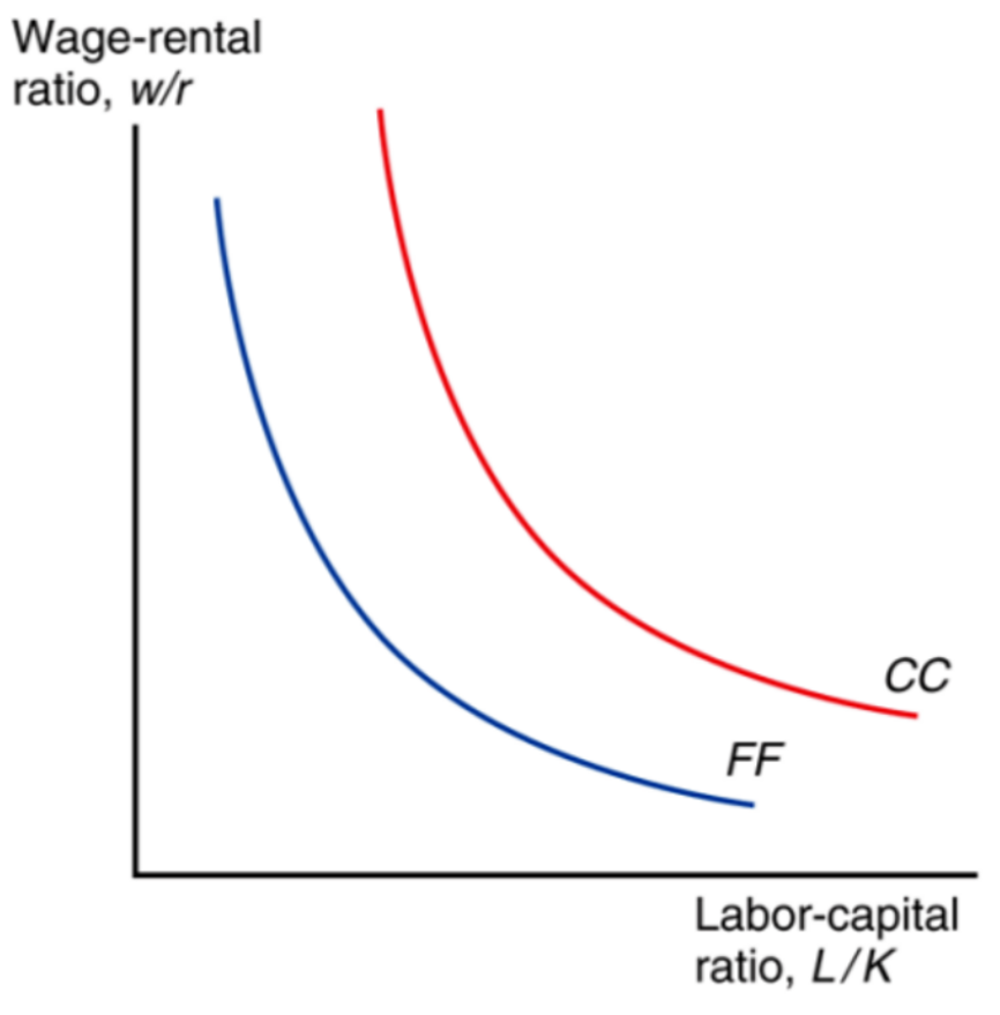
\includegraphics[scale=.8]{ho_factor_intensity}
  \end{figure}
\end{frame}
%--------------------------------------

%--------------------------------------
\begin{frame}{PPF with factor substitution}
  \begin{figure}
    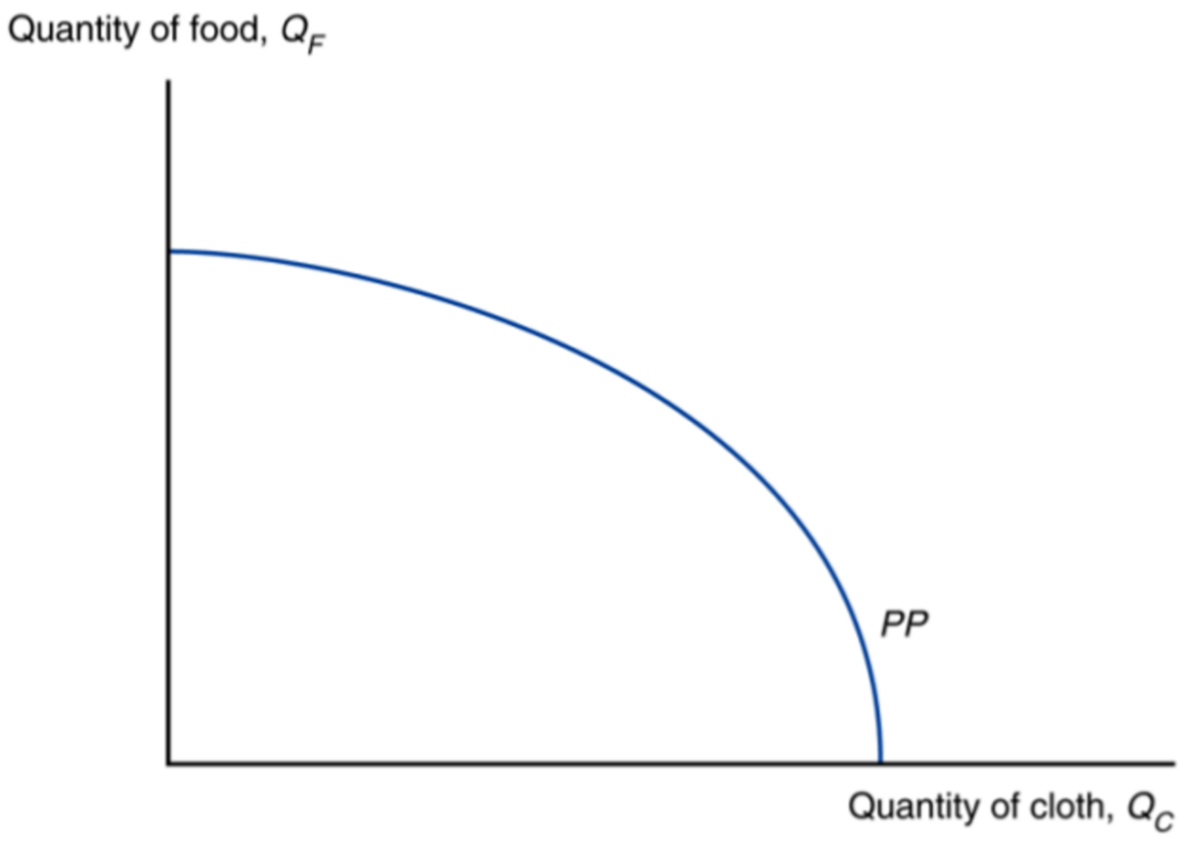
\includegraphics[scale=.8]{ho_ppf}
  \end{figure}  
\end{frame}
%--------------------------------------

%--------------------------------------
\begin{frame}
  The output price ratio is given by
  \begin{align*}
    \frac{p_c}{p_f}=\frac{MPL_f}{MPL_c}=\frac{MPK_f}{MPK_c}
  \end{align*}
  Production will be a given point on the PPF tangent to
  \begin{align*}
  -\frac{p_c}{p_f}
  \end{align*}
  \medskip   
  The economy will produce at a point that maximises the value of production $V$  
  \begin{align*}
    V=p_cQ_c+p_fQ_f
  \end{align*}
\end{frame}
%--------------------------------------

%--------------------------------------
\begin{frame}{Production function}
  \begin{figure}
    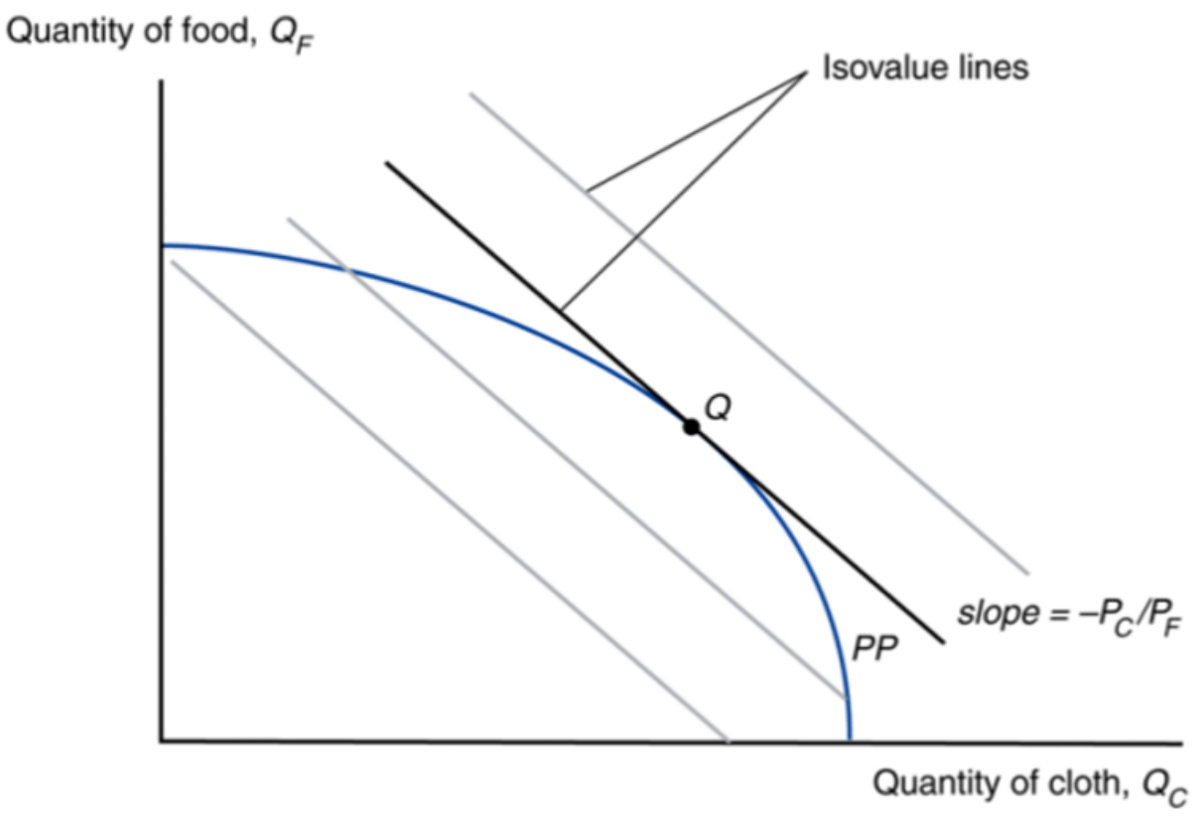
\includegraphics[scale=.8]{ho_production}
  \end{figure}
\end{frame}
%--------------------------------------

%--------------------------------------
\begin{frame}
  Wage and capital rate are given by
  \begin{align*}
  w &= p_c\cdot MPL_c = p_f \cdot MPL_f\\
  r &= p_c \cdot MPK_c = p_f \cdot MPK_f
  \end{align*}
Therefore, relative factor prices are given by
  \begin{align*}
    \frac{w}{r}=\frac{MPL_c}{MPK_c}=\frac{MPL_f}{MPK_c}
  \end{align*}
  Production will be a given point on the PPF tangent to 
  \begin{align*}
  -\frac{w}{r}
  \end{align*}  
  i.e. as $w$ increases relative to $r$ producers will use less labour and more capital     
\end{frame}
%--------------------------------------

%--------------------------------------
\begin{frame}
  Concerning the mix of inputs we have that
  \begin{align*}
    \frac{a_{lc}}{a_{kc}} > \frac{a_{lf}}{a_{kf}}\\
    \frac{L_c}{K_c} > \frac{L_f}{K_f}
  \end{align*}
  i.e cloth production is relatively labour intensive whereas food production is relatively capital intensive.
\end{frame}
%--------------------------------------

%--------------------------------------
\begin{frame}{Recall factor intensity}
  \begin{figure}
    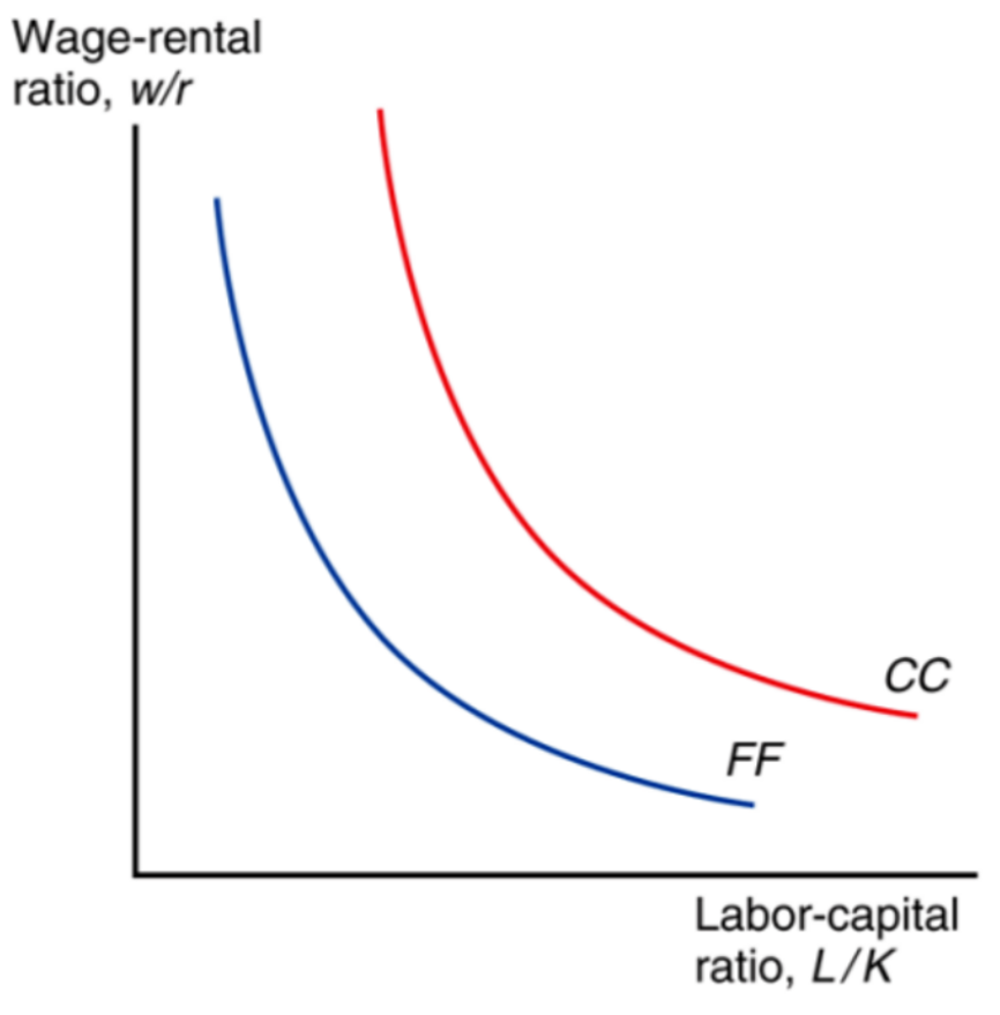
\includegraphics[scale=.8]{ho_factor_intensity}
  \end{figure}
\end{frame}
%--------------------------------------

%--------------------------------------
\begin{frame}
  With regard to resource use and production possibilities, let's assume a scenario where the economy's labour force grows.
  What will happen to
  \begin{enumerate}
    \item The labour to capital ratio?
    \item Production possibilities
    \item Ratio of labour to capital ratio used in both sectors
  \end{enumerate}
\end{frame}
%--------------------------------------

%--------------------------------------
\begin{frame}
  \begin{enumerate}
    \item The labour to capital ratio will expand
    \item Expansion of production possibilities is biased towards cloth, which is labour intensive
    \item Ratio of labour to capital used remains constant given relative cloth price
  \end{enumerate}
  So to employ the additional workers, the economy expand the production of the relatively labour intensive good and contracts the production of the relative capital intensive good.
\end{frame}
%--------------------------------------

%--------------------------------------
\begin{frame}{Resources and production possibilities}
  \begin{figure}
    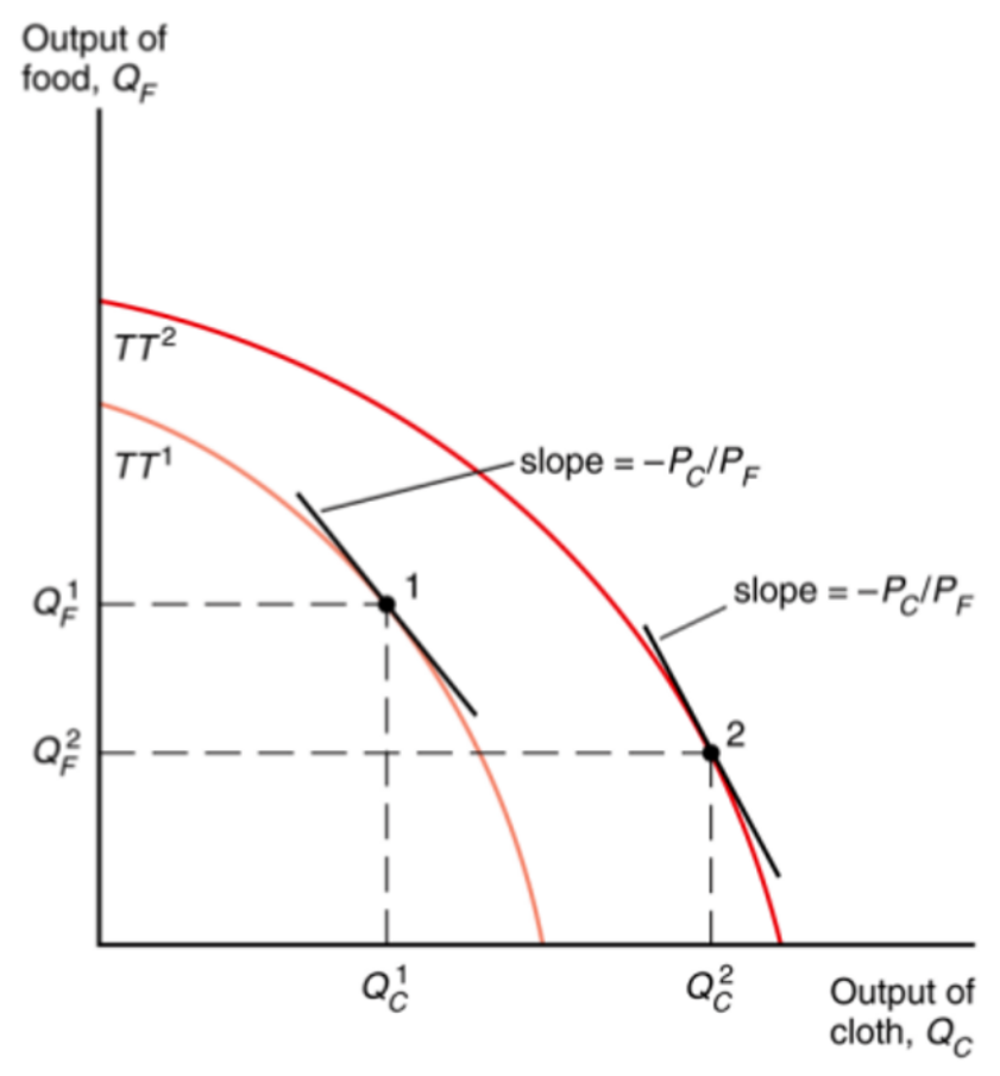
\includegraphics[scale=.8]{ho_ppf2}
  \end{figure}
\end{frame}
%--------------------------------------


%--------------------------------------
\begin{frame}
  Prices are determined by
  \begin{align*}
    p_c = a_{lc} \cdot w + a_{kc} \cdot r\\
    p_f = a_{lf} \cdot w + a_{kf} \cdot r
  \end{align*}
  \medskip
  Under competition, the commodity price equals the production cost which depends on
  \begin{itemize}
    \item Wages paid to labour $w$ and rents to capital $r$
    \item Units of labour and capital used
  \end{itemize}
  \medskip
  Effect of change in $w,r$ on production costs depends on mix of factors used.
  \begin{itemize}
    \item Change in $\frac{w}{r}$ tied to changes in $\frac{p_c}{p_f}$
  \end{itemize}  
\end{frame}
%--------------------------------------

%--------------------------------------
\begin{frame}
  \textbf{Stolper-Samuelson theorem}
  \begin{quote}
   An increase in the relative price of a good will increase the relative remuneration of the factor which is intensively used in the production of this good and reduces the remuneration of the other factor. 
  \end{quote}
  \medskip
  i.e. a price change in output goods will hurt some input owners.\\
  Theorem links input and output prices.
  \begin{itemize}
      \item Trade will change output prices: some people are hurt by trade
  \end{itemize}  
\end{frame}
%--------------------------------------

%--------------------------------------
\begin{frame}{Factor and commodity prices}
  \begin{figure}
    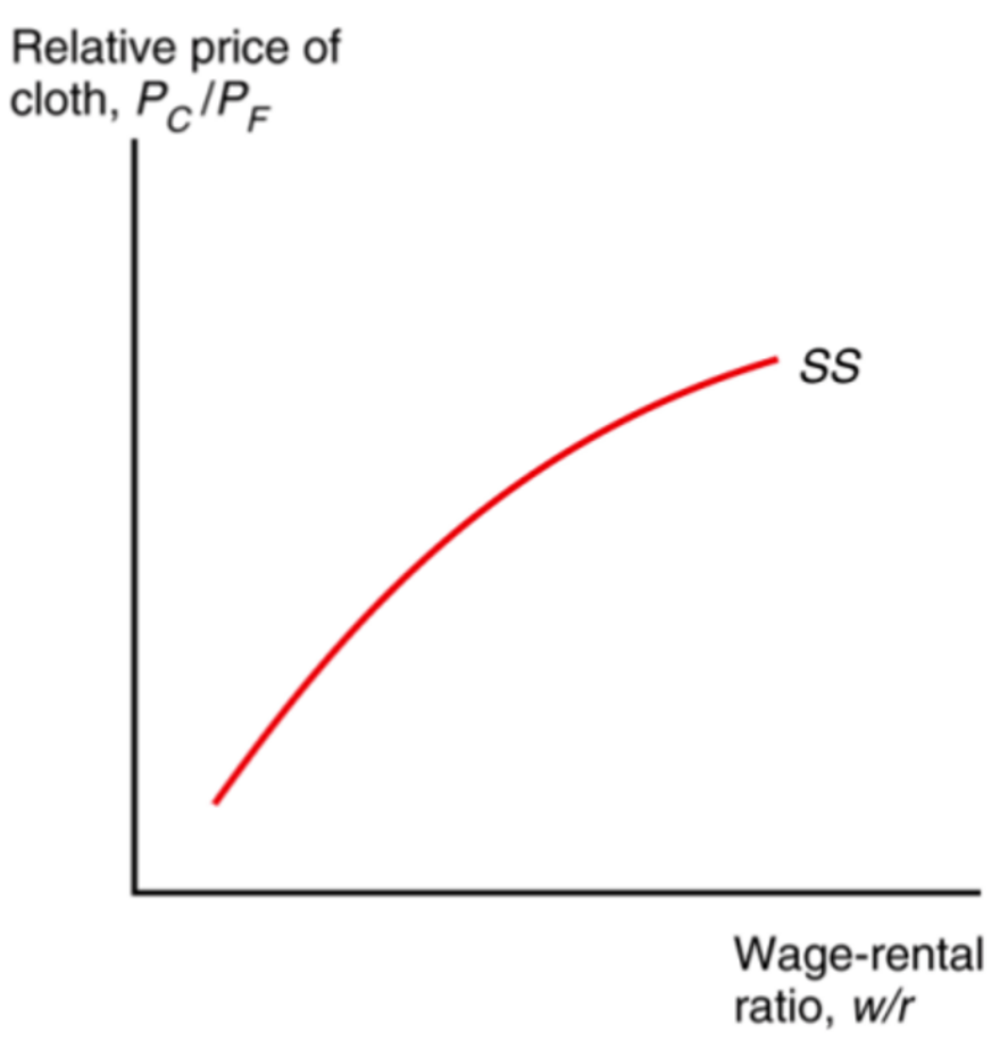
\includegraphics[scale=.8]{ho_prices}
  \end{figure}
\end{frame}
%--------------------------------------

%--------------------------------------
\begin{frame}{Commodity prices and input choices}
  \begin{figure}
    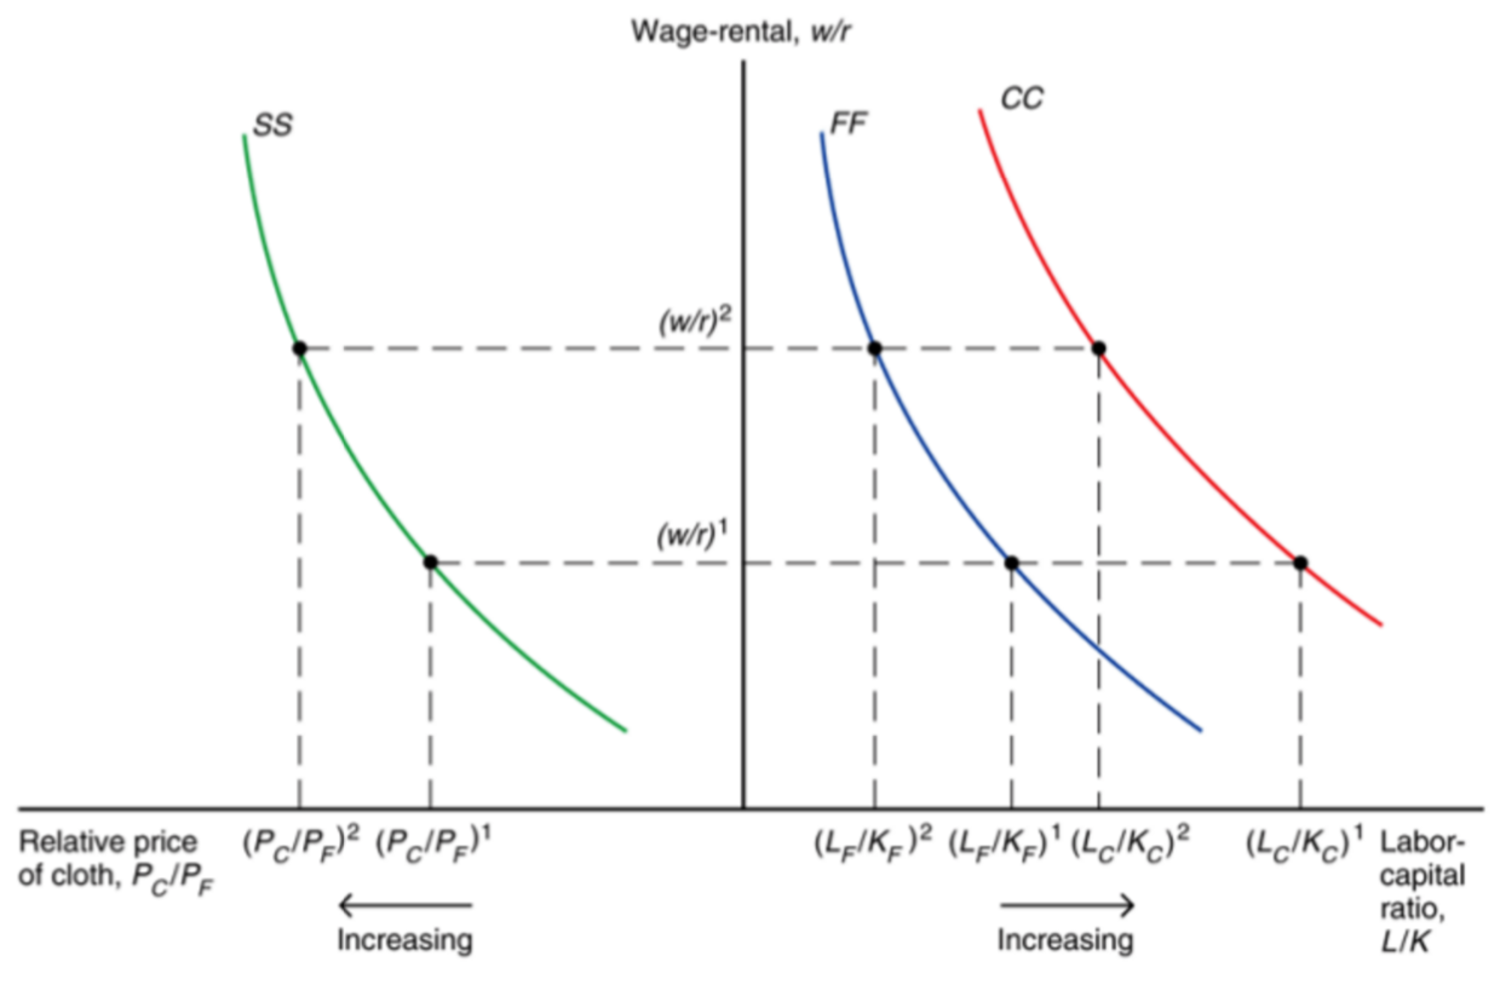
\includegraphics[scale=.8]{ho_inputs}
  \end{figure}
\end{frame}
%--------------------------------------

%--------------------------------------
\begin{frame}
  Under the Stolper-Samuelson theorem, opening up to trade will lead to
  \begin{enumerate}
    \item Rise in real remuneration of relatively abundant factor
    \item Fall in real remuneration of relative scarce factor
  \end{enumerate}
  \medskip
  Therefore trade will create winners and losers. 
  \begin{itemize}
    \item In our example $Home$ capital owners and $Foreign$ labourers won't be happy.
  \end{itemize}
  \medskip
  The government can implement policy such that losers can be compensated through fiscal transfers from winners. 
\end{frame}
%--------------------------------------

%--------------------------------------
  \begin{frame}{Compensating trade losers}
\framesubtitle{source: OECD}
  \begin{figure}
    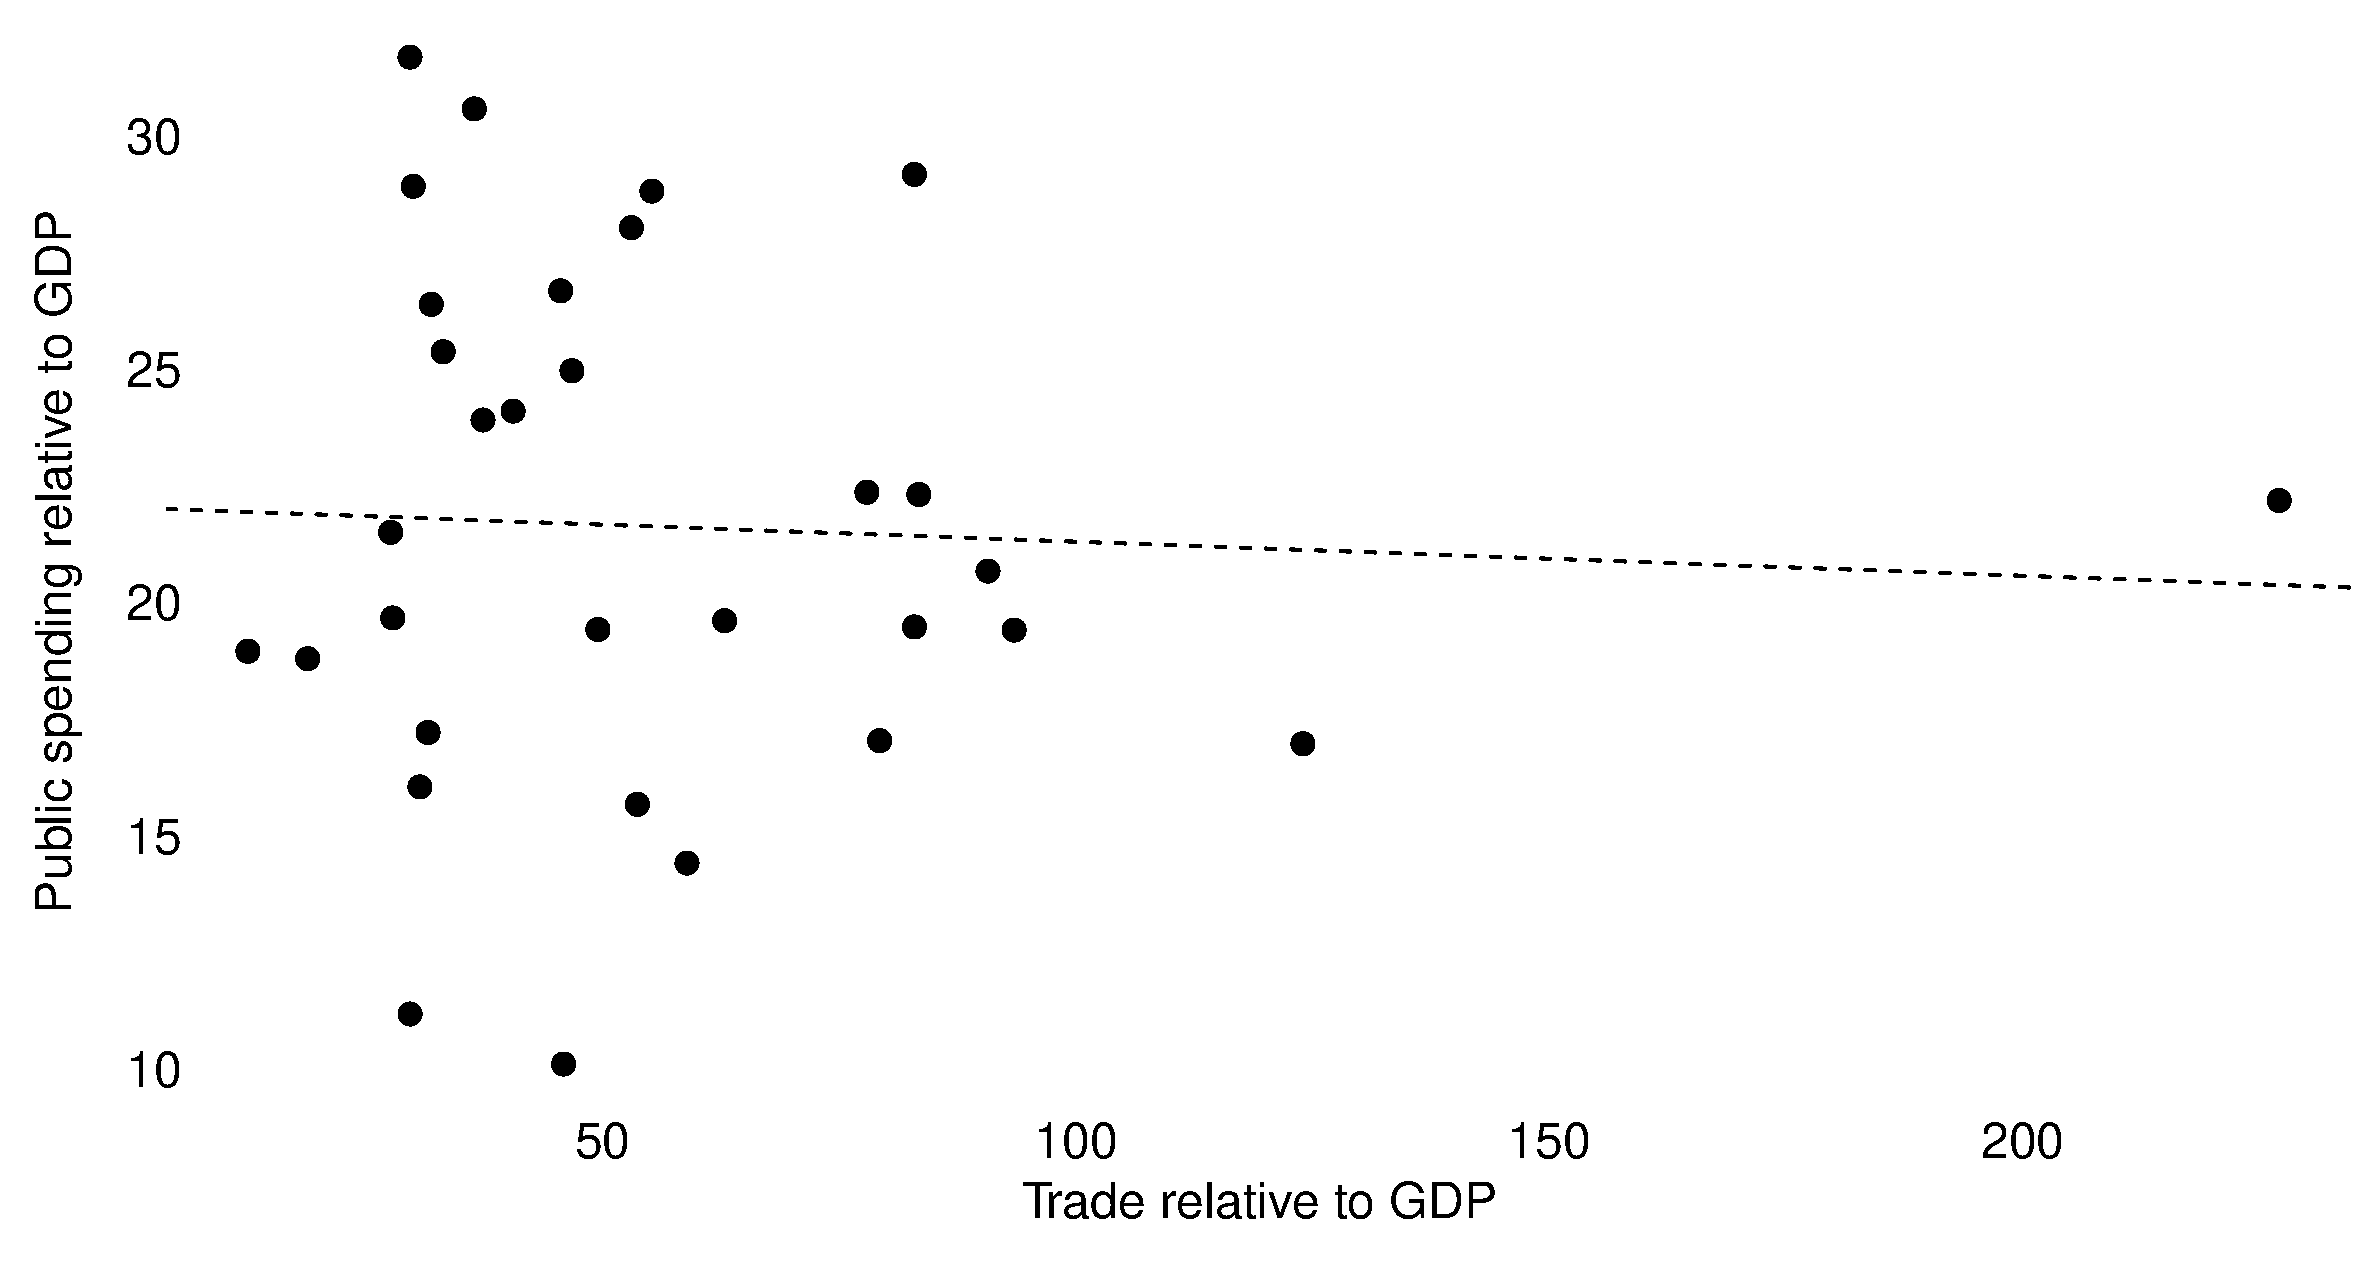
\includegraphics[scale=.25]{compensation}
  \end{figure}
\end{frame}
%--------------------------------------

%--------------------------------------
\begin{frame}
  \textbf{Rybczynski theorem}
  \begin{quote}
  For a given relative price, a higher endowment in one factor makes the production that uses this factor more intensively increase and the production that uses it less intensively decrease.  
  \end{quote}
\end{frame}
%--------------------------------------

%--------------------------------------
\begin{frame}{An increase in capital}
  \begin{figure}
    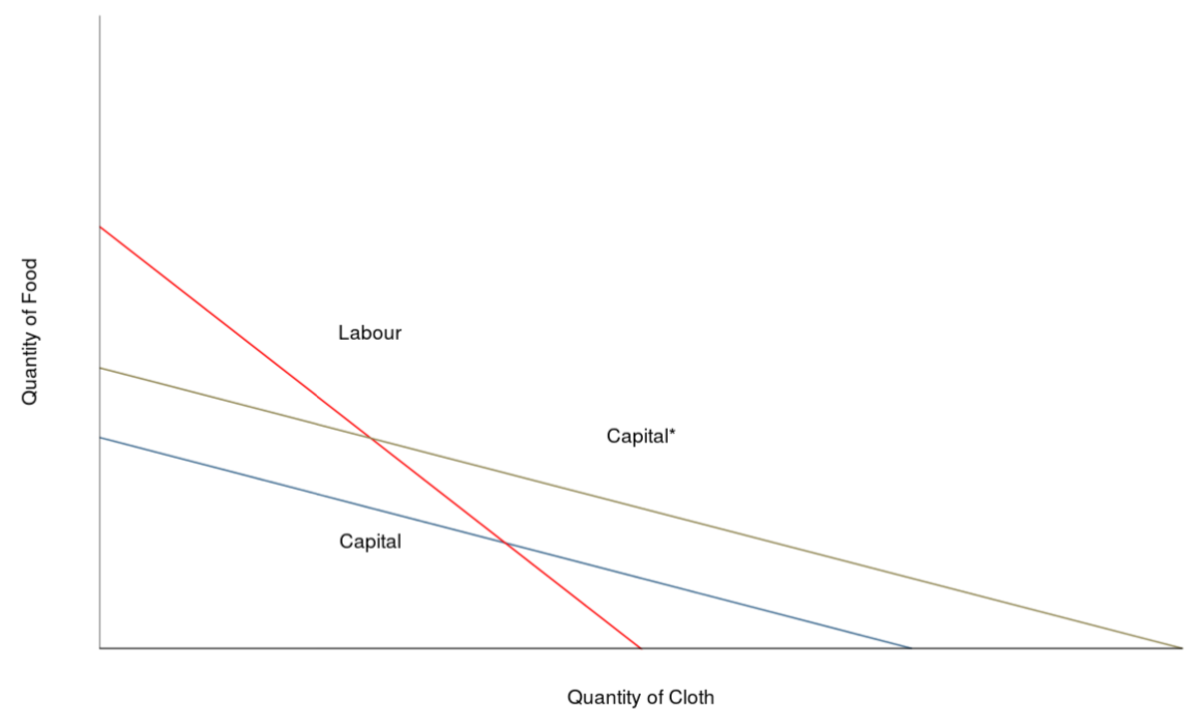
\includegraphics{ryb}
  \end{figure}  
\end{frame}
%--------------------------------------

%--------------------------------------
\begin{frame}
 Following the Rybczynski theorem, the effect of the higher endowment on the trading economy depends on the size of the economy. 
For a small economy an increase in factor endowments is beneficial since it can lead to 
  \begin{enumerate}
    \item Export-biased growth: can export/import more, and thus consume more 
    \item Import-substitution growth: can import/export less, but still consume more 
  \end{enumerate}
\end{frame}
%--------------------------------------

%--------------------------------------
\begin{frame}{Source: Romalis (2003)}
  \begin{figure}
    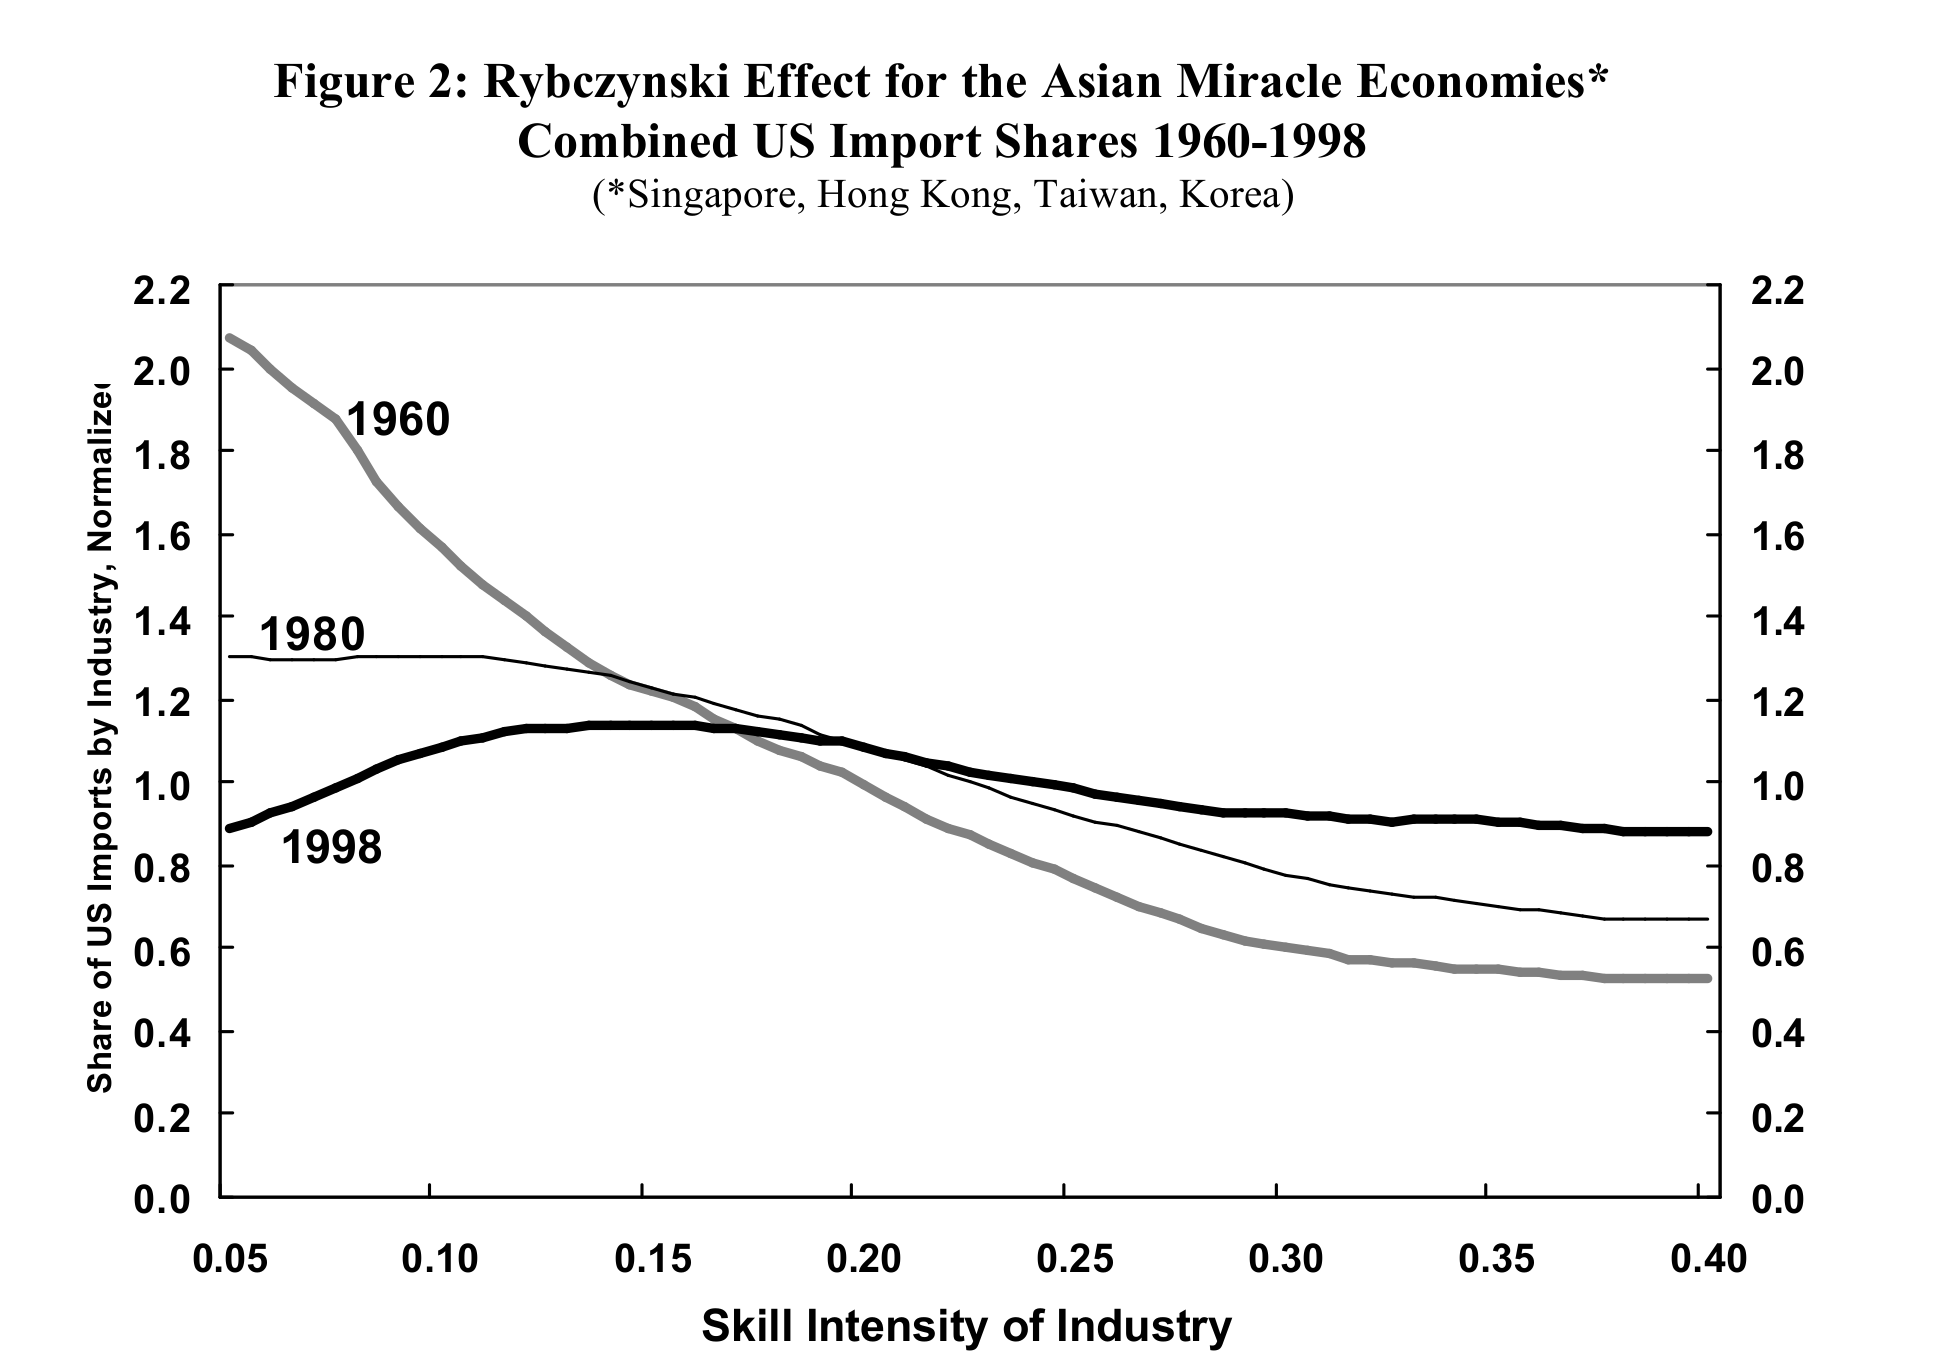
\includegraphics[scale=.7]{ho_research2.png}
  \end{figure}
\end{frame}
%--------------------------------------

%--------------------------------------
\begin{frame}
  In contrast, for a large economy an increase in factor endowment could have adverse effects since prices are endogenous
  \begin{itemize}
    \item e.g. Brazil is a price-setter in the coffee industry
  \end{itemize}
  \medskip
  The deterioration of terms-of-trade through export-biased growth might offset the positive impact of the higher endowments. 
  This effect of impoverishing growth can serve as a justification for import-substitution policies.
\end{frame}
%--------------------------------------

%--------------------------------------
\begin{frame}
  Concerning trade patterns recall that both countries have the same technology level, and $Home$ is relatively labour abundant.
  \begin{align*}
    \frac{Q_c}{Q_f} > \frac{Q_c^*}{Q_f^*}
  \end{align*}
  Therefore $Home$ will export the relatively more labour intensive good.
  Consumption will depend on the output price and the equilibrium consumption ratio is given by
  \begin{align*}
    \frac{D_c}{D_f} = \frac{D_c^*}{D_f^*}
  \end{align*}
\end{frame}
%--------------------------------------

%--------------------------------------
\begin{frame}
  \textbf{Heckscher-Ohlin theorem}
  \begin{quote}
   Countries with relatively more of a resource will export goods for which that resource is more useful in production. 
  \end{quote}
  i.e. more capital means exporting capital intensive goods, more labour means exporting more labour intensive goods.
\end{frame}
%--------------------------------------

%--------------------------------------
\begin{frame}
  The HO-model predicts convergence of relative prices following trade, similar to the Ricardian model.\\
  The relative prices will change in favour of the abundant resource in each country.
  For example the price of cloth will
  \begin{itemize}
    \item Increase in the relatively labour abundant country
    \item Decrease in the relatively labour scarce country
  \end{itemize}
\end{frame}
%--------------------------------------

%--------------------------------------
\begin{frame}{Convergence of relative prices}
  \begin{figure}
    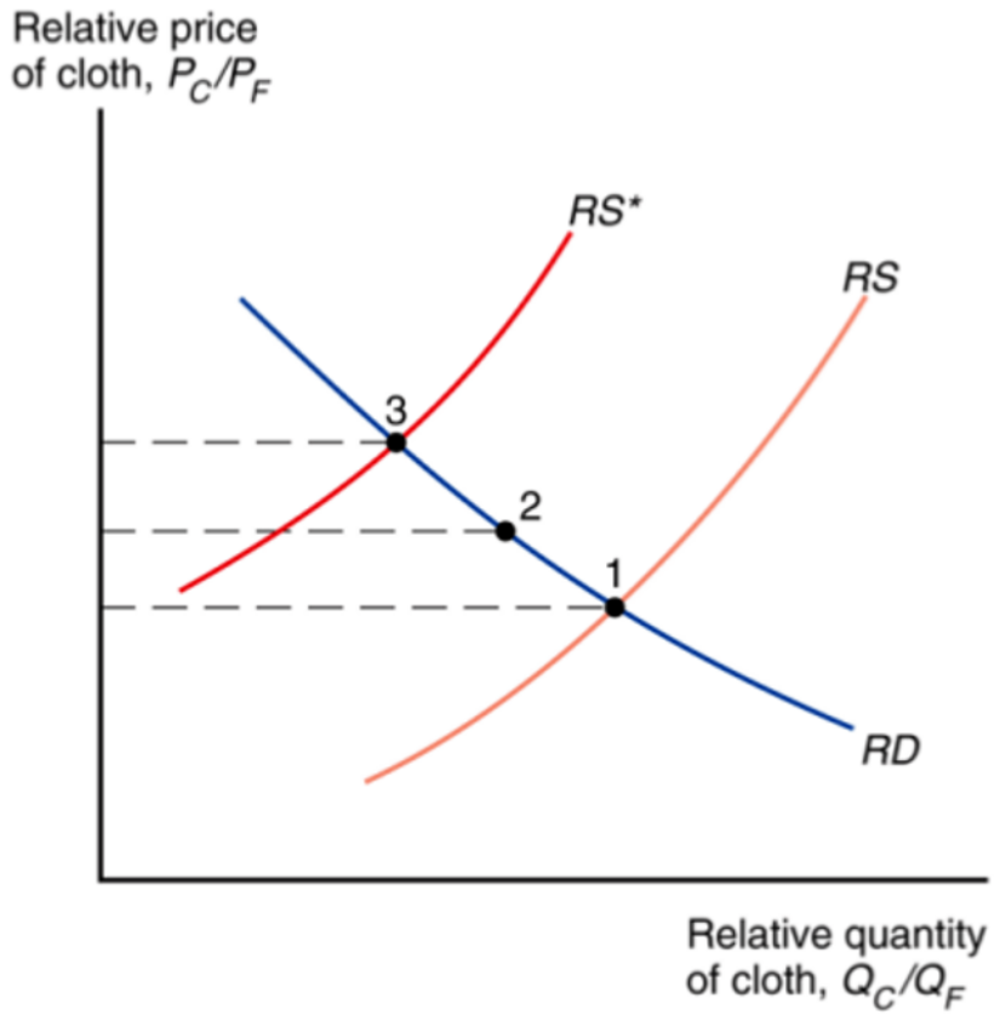
\includegraphics[scale=.9]{ho_rprices}
  \end{figure}
\end{frame}
%--------------------------------------

%--------------------------------------
\begin{frame}
  In our example model, opening up to trade will increase the relative price of cloth meaning that $Home$ 
  \begin{itemize}
    \item Will increase production and decrease consumption
    \item Become a cloth exporter and food importer
  \end{itemize}
  This also entails that $Foreign$ will export food and import cloth.
\end{frame}
%--------------------------------------

%--------------------------------------
\begin{frame}
  Concerning factor price equalisation the HO-model predicts equalisation among countries that trade, in contrast with the Ricardian model. 
  \begin{enumerate}
    \item Free trade equalises relative output prices
    \item Stolper-Samuelson theorem links output and factor prices, so factor prices are equalised
  \end{enumerate}
  Trade will also increase the price of relatively abundant factors as there is an increase in the demand for the goods produced by these factors.
\end{frame}
%--------------------------------------

%--------------------------------------
\begin{frame}
  According to the Heckscher-Ohlin model trade is likely to reduce global income inequality.\\
  Consider two factors
  \begin{enumerate}
    \item Skilled labour
    \item Unskilled labour
  \end{enumerate} 
  \medskip
  In this case trade liberalisation should lead to imports of goods intensive in unskilled labour in a skilled-labour abundant country.   
  \begin{itemize}
    \item This leads to an increase in the relative price of goods intensive in unskilled labour
    \item And increases the returns to unskilled labour relative to skilled labour
  \end{itemize}
  \medskip
  The result of this process is a reduction in wage inequality.\footnote{Across countries.} 
\end{frame}
%--------------------------------------

%--------------------------------------
\begin{frame}{Source: Romalis (2003)}
  \begin{figure}
    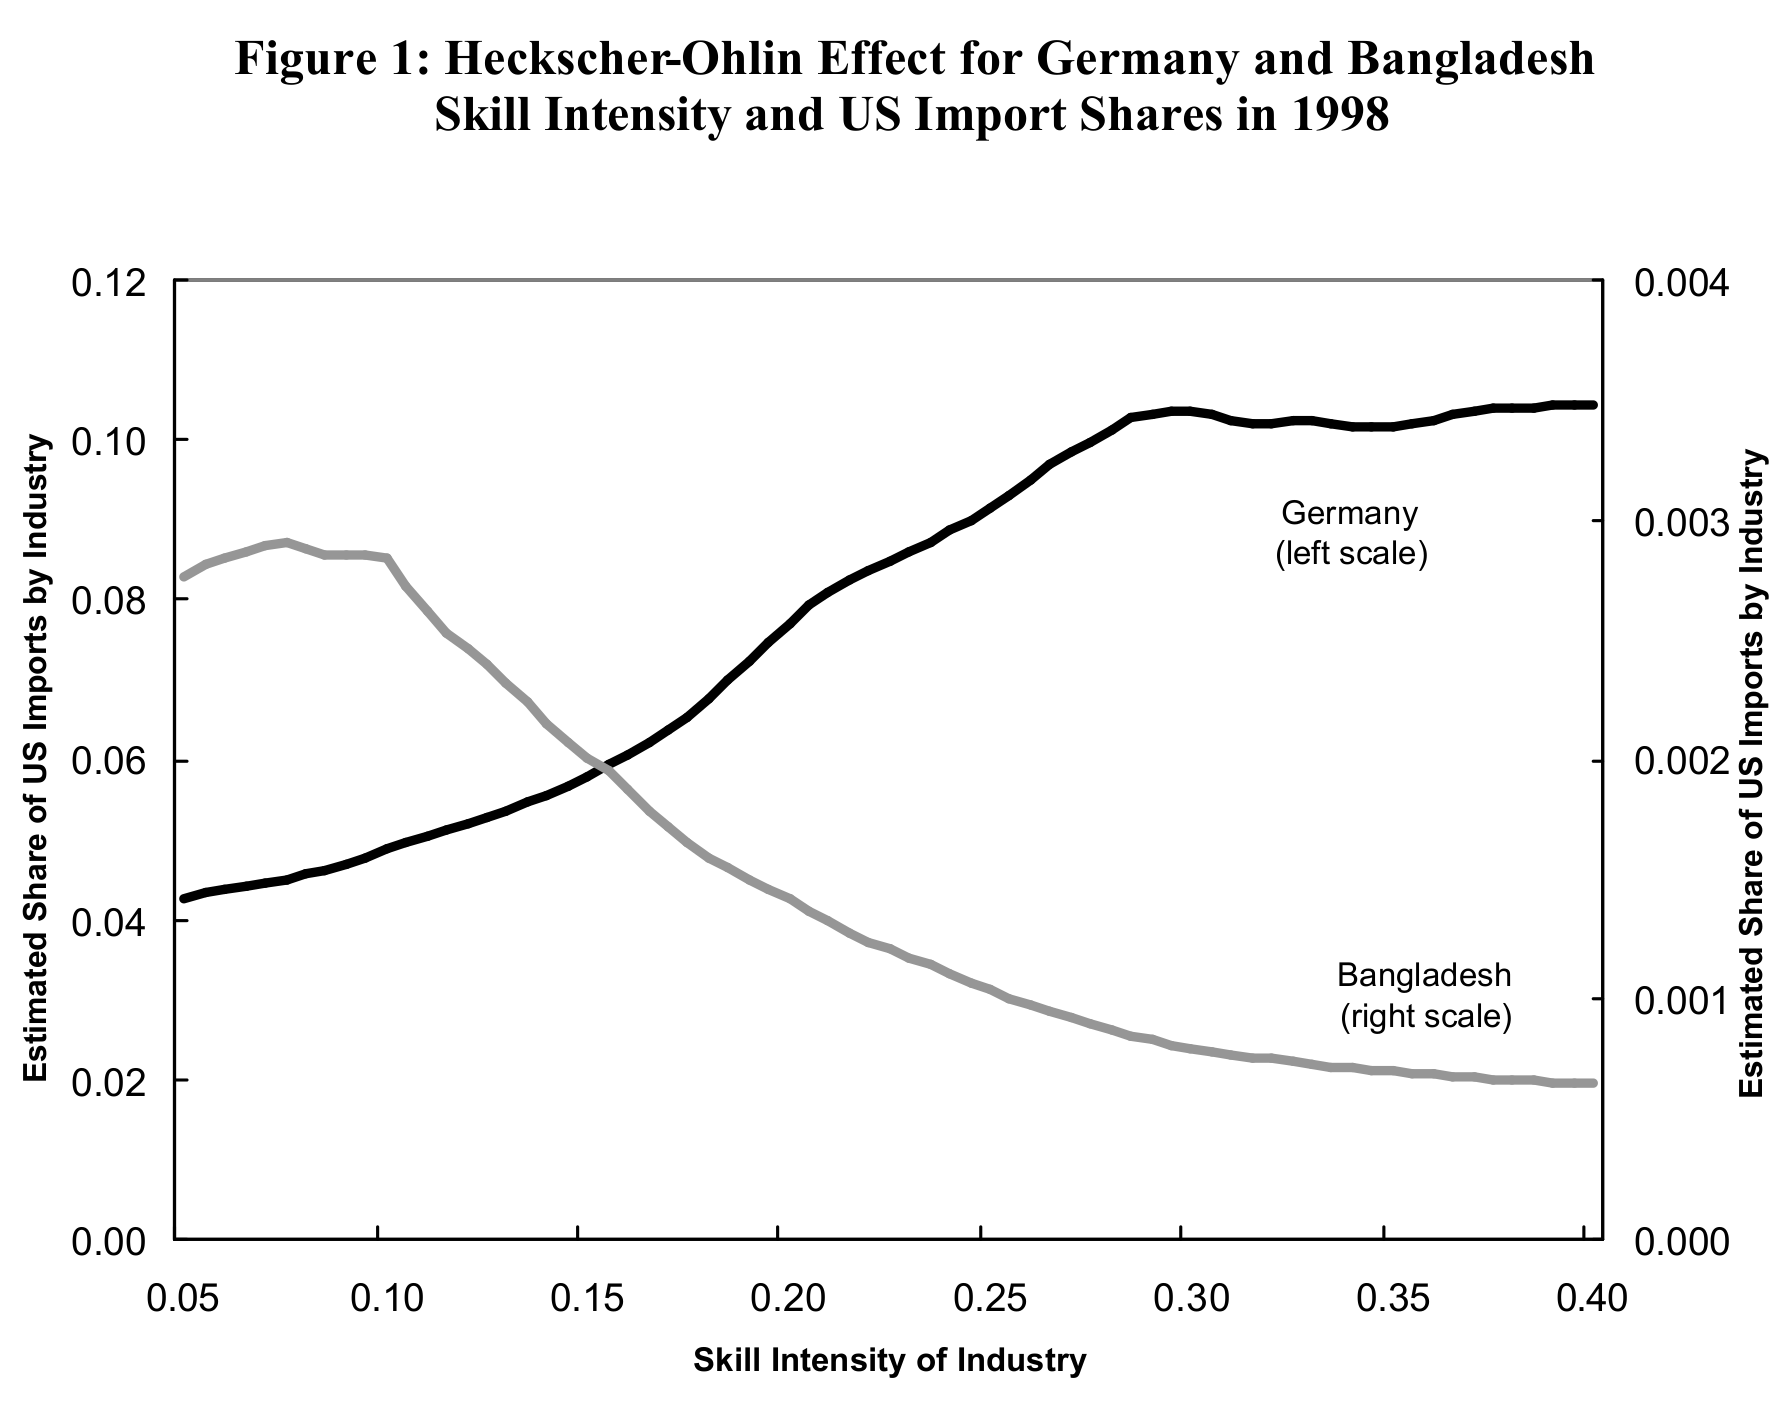
\includegraphics[scale=.7]{ho_research.png}
  \end{figure}
\end{frame}
%--------------------------------------

%--------------------------------------
\begin{frame}{Absence of wage equalisation across countries}
\framesubtitle{source: US Bureau of Labor Statistics}
  \begin{figure}
    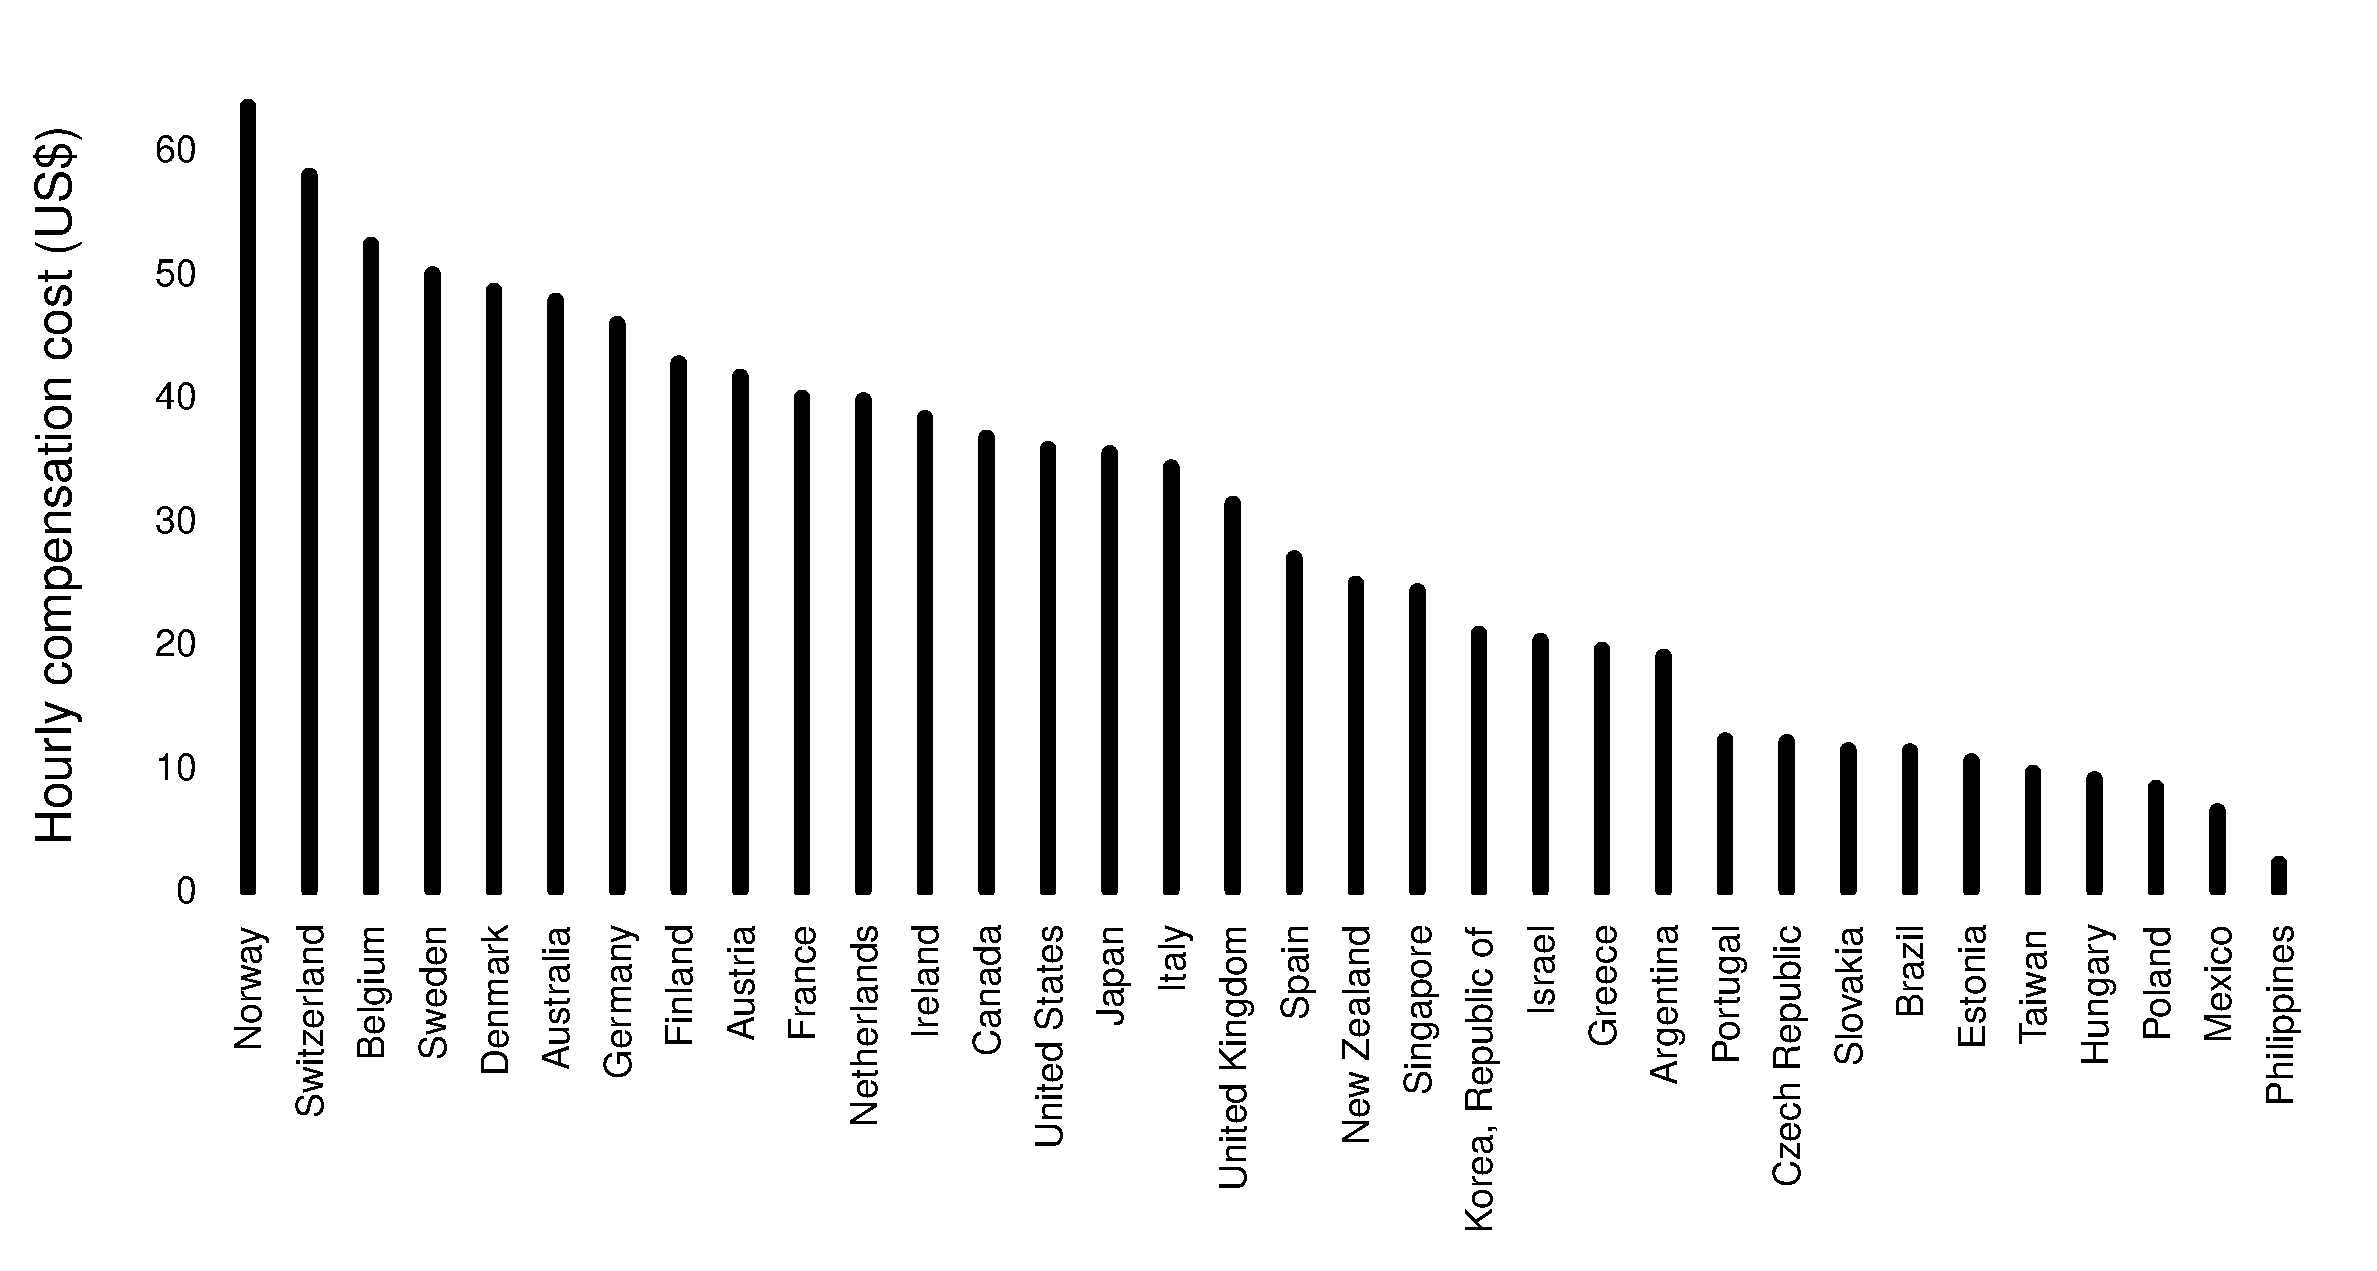
\includegraphics[scale=.25]{wages}
  \end{figure}
\end{frame}
%--------------------------------------

%--------------------------------------
\begin{frame}{No Great Equalisation}
\framesubtitle{source: Leamer (2007)}
  \begin{figure}
    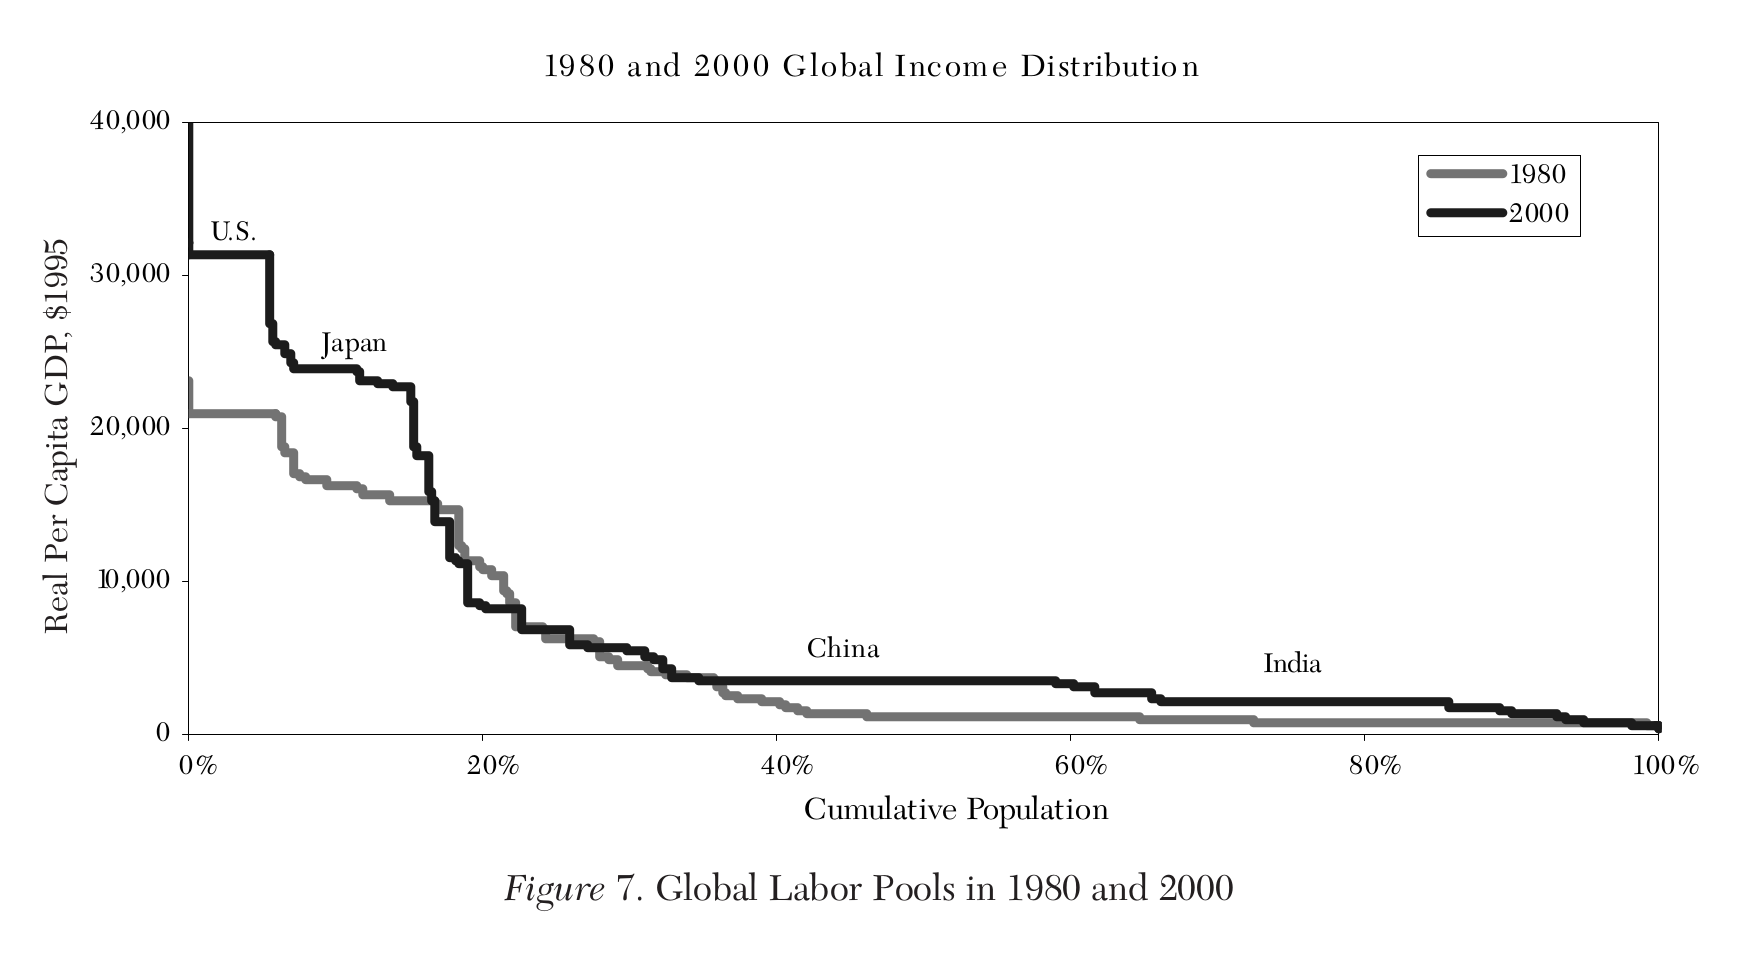
\includegraphics[scale=.7]{leamer}
  \end{figure}
\end{frame}
%--------------------------------------

%--------------------------------------
\begin{frame}
 Opening up to trade we would expect to see wage equalise according to the factor price equalisation theorem.
 Why isn't this happening?
 \medskip
 \begin{enumerate}
   \item In real life free trade does not exist
   \item Distortion through monopolies, labour unions, government policy
   \item Constant returns to scale might not hold
   \item Technologies are not the same across countries
   \item Labour and capital are not homogenous
 \end{enumerate}
\end{frame}
%--------------------------------------

%--------------------------------------
\begin{frame}
 One advantage of the HO-model is that it is relatively straightforward to analyse graphically which can be done using the Lerner diagram. 
 \begin{itemize}
   \item The diagram relates goods and factor prices for the HO-model
 \end{itemize}
 \medskip
 A distinguishing feature of this type of diagram is that it used unit-value isoquants.
\end{frame}
%--------------------------------------

%--------------------------------------
\begin{frame}
 Let's start with a simple example of an economy with a single sector that produces good $X$ using inputs $K$ and $L$
 \begin{itemize}
   \item We assume constant returns to scale.
 \end{itemize}
 \medskip
The diagrams in the next slides will show two lines
\begin{enumerate}
  \item isocost line: combination of $K$ and $L$ that costs 1 euro
  \item isoquant line: combination of $K$ and $L$ that produces 1 euro $X$
\end{enumerate}
\medskip
The unit-value isoquant and isocost are given by
\begin{align*}
X &=\frac{1}{p_x}\\
rK+wL&=1
\end{align*}
\medskip
The country has endowments $E$.
\end{frame}
%--------------------------------------

%--------------------------------------
\begin{frame}
  \begin{figure}
    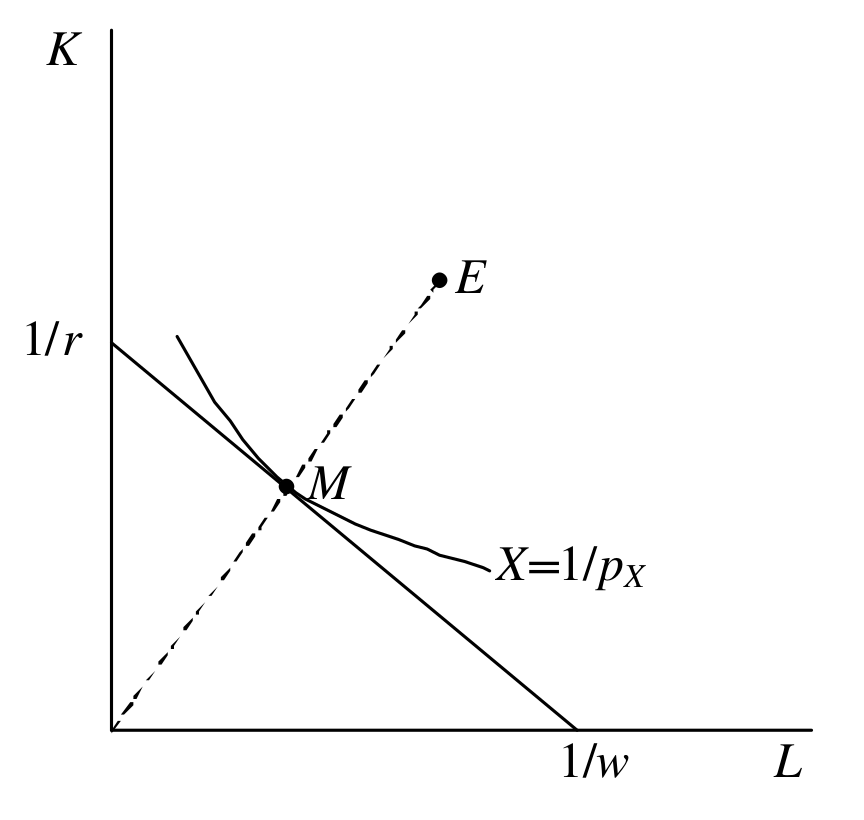
\includegraphics{lerner.png}
  \end{figure}
\end{frame}
%--------------------------------------

%--------------------------------------
\begin{frame}
We can change the endowment level proportionally $E'$ or increase labour $E''$
  \begin{figure}
    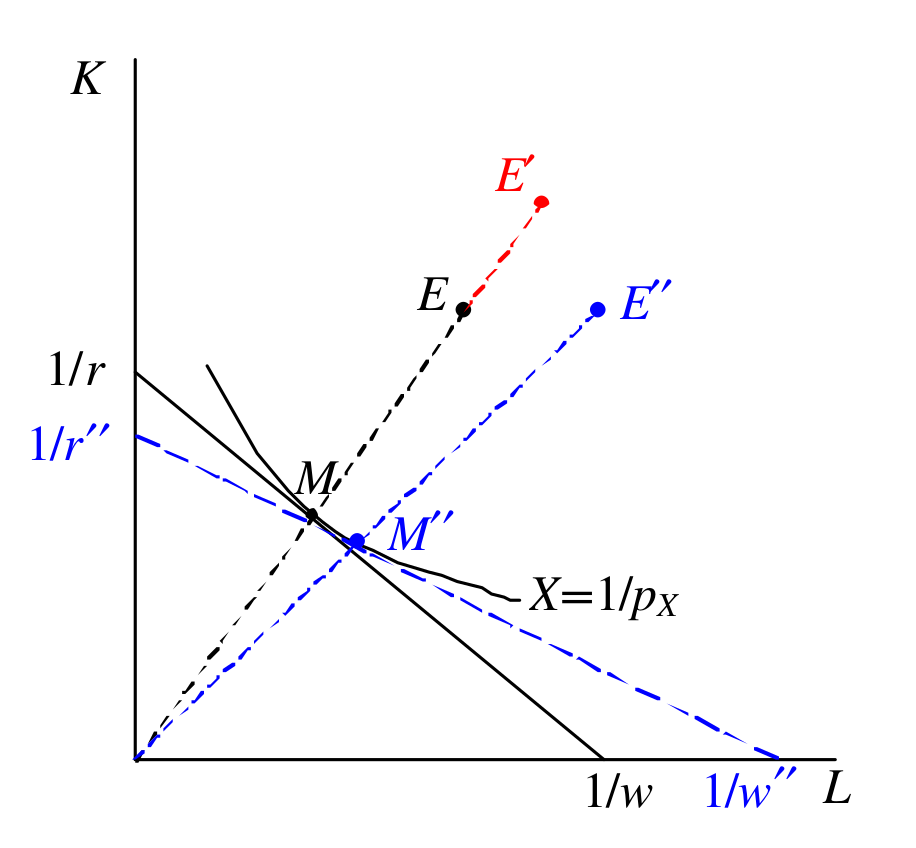
\includegraphics[scale=.7]{lerner2.png}    
  \end{figure}
\end{frame}
%--------------------------------------

%--------------------------------------
\begin{frame}
Let's consider an economy with two sectors, $X$ and $Y$, with prices $p_x$ and $p_y$.
  \begin{figure}
    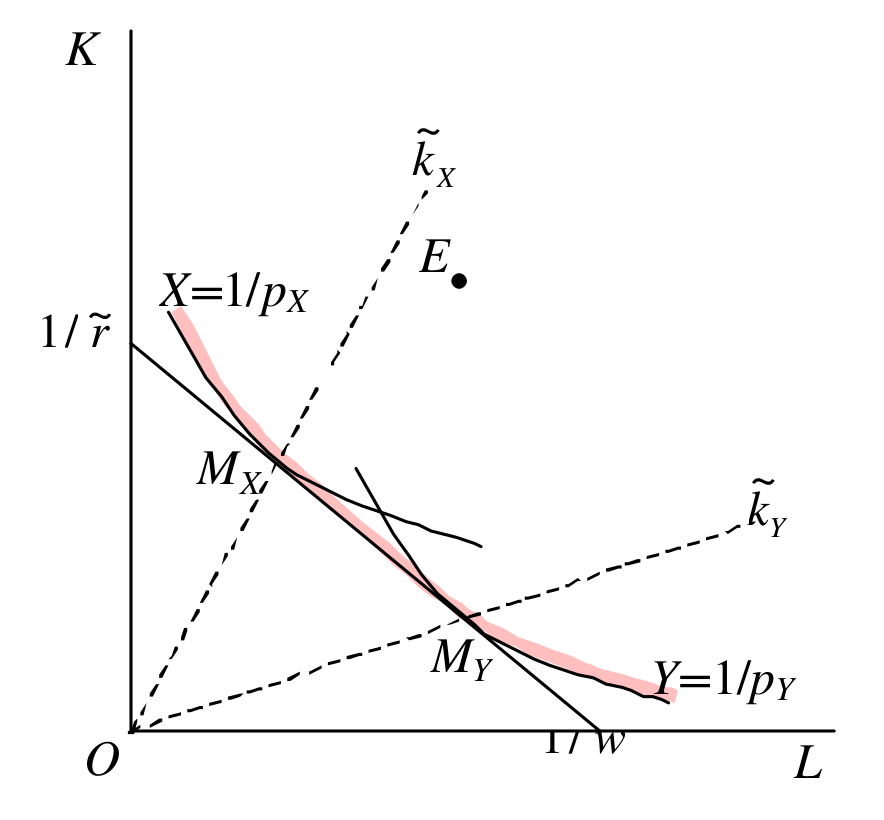
\includegraphics[scale=.7]{lerner3.png}
  \end{figure}
\end{frame}
%--------------------------------------

%--------------------------------------
\begin{frame}
 From the figure it follows that for factor endowments within the cone factor prices must be same.
 Consider two countries under free trade with
 \begin{itemize}
   \item The same technologies
   \item Similar endowment levels
   \item Facing the same world prices
 \end{itemize}
They will end up in the same diversification cone, meaning that thay have the same factor prices.
This is the central message of the \textbf{factor price equalisation} theorem. 
\end{frame}
%--------------------------------------

%--------------------------------------
\begin{frame}
  Can include the Edgeworth box in the diagram.
  \begin{figure}
    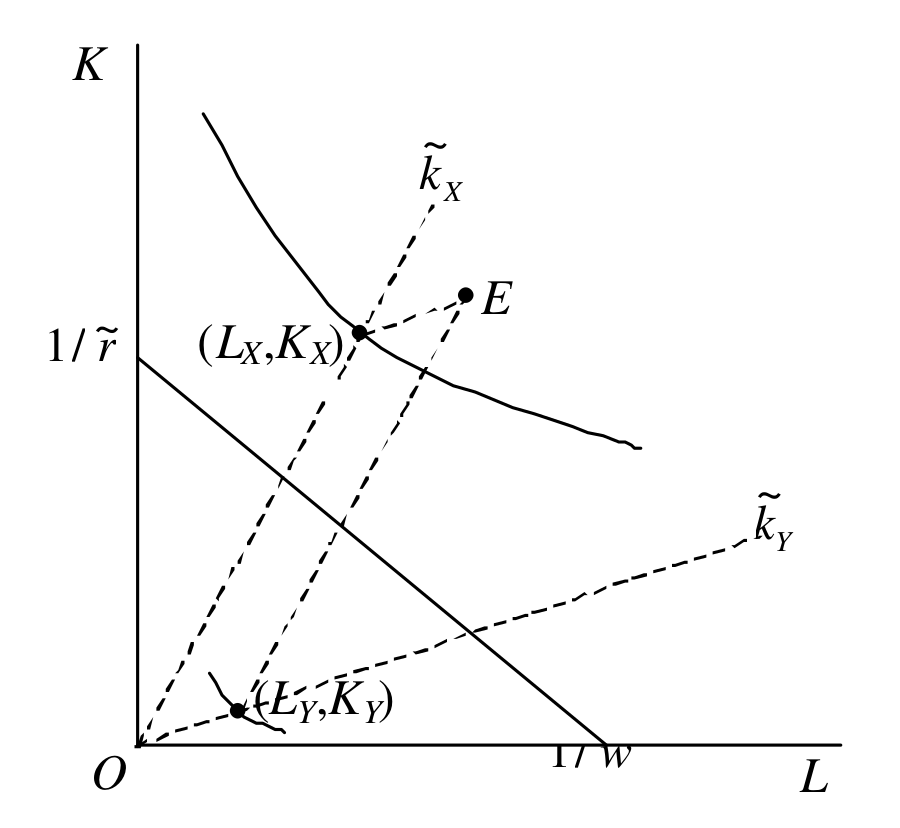
\includegraphics[scale=.7]{lerner4.png}
  \end{figure}
\end{frame}
%--------------------------------------

%--------------------------------------
\begin{frame}{Example: how to draw a Lerner diagram}
  \begin{figure}
    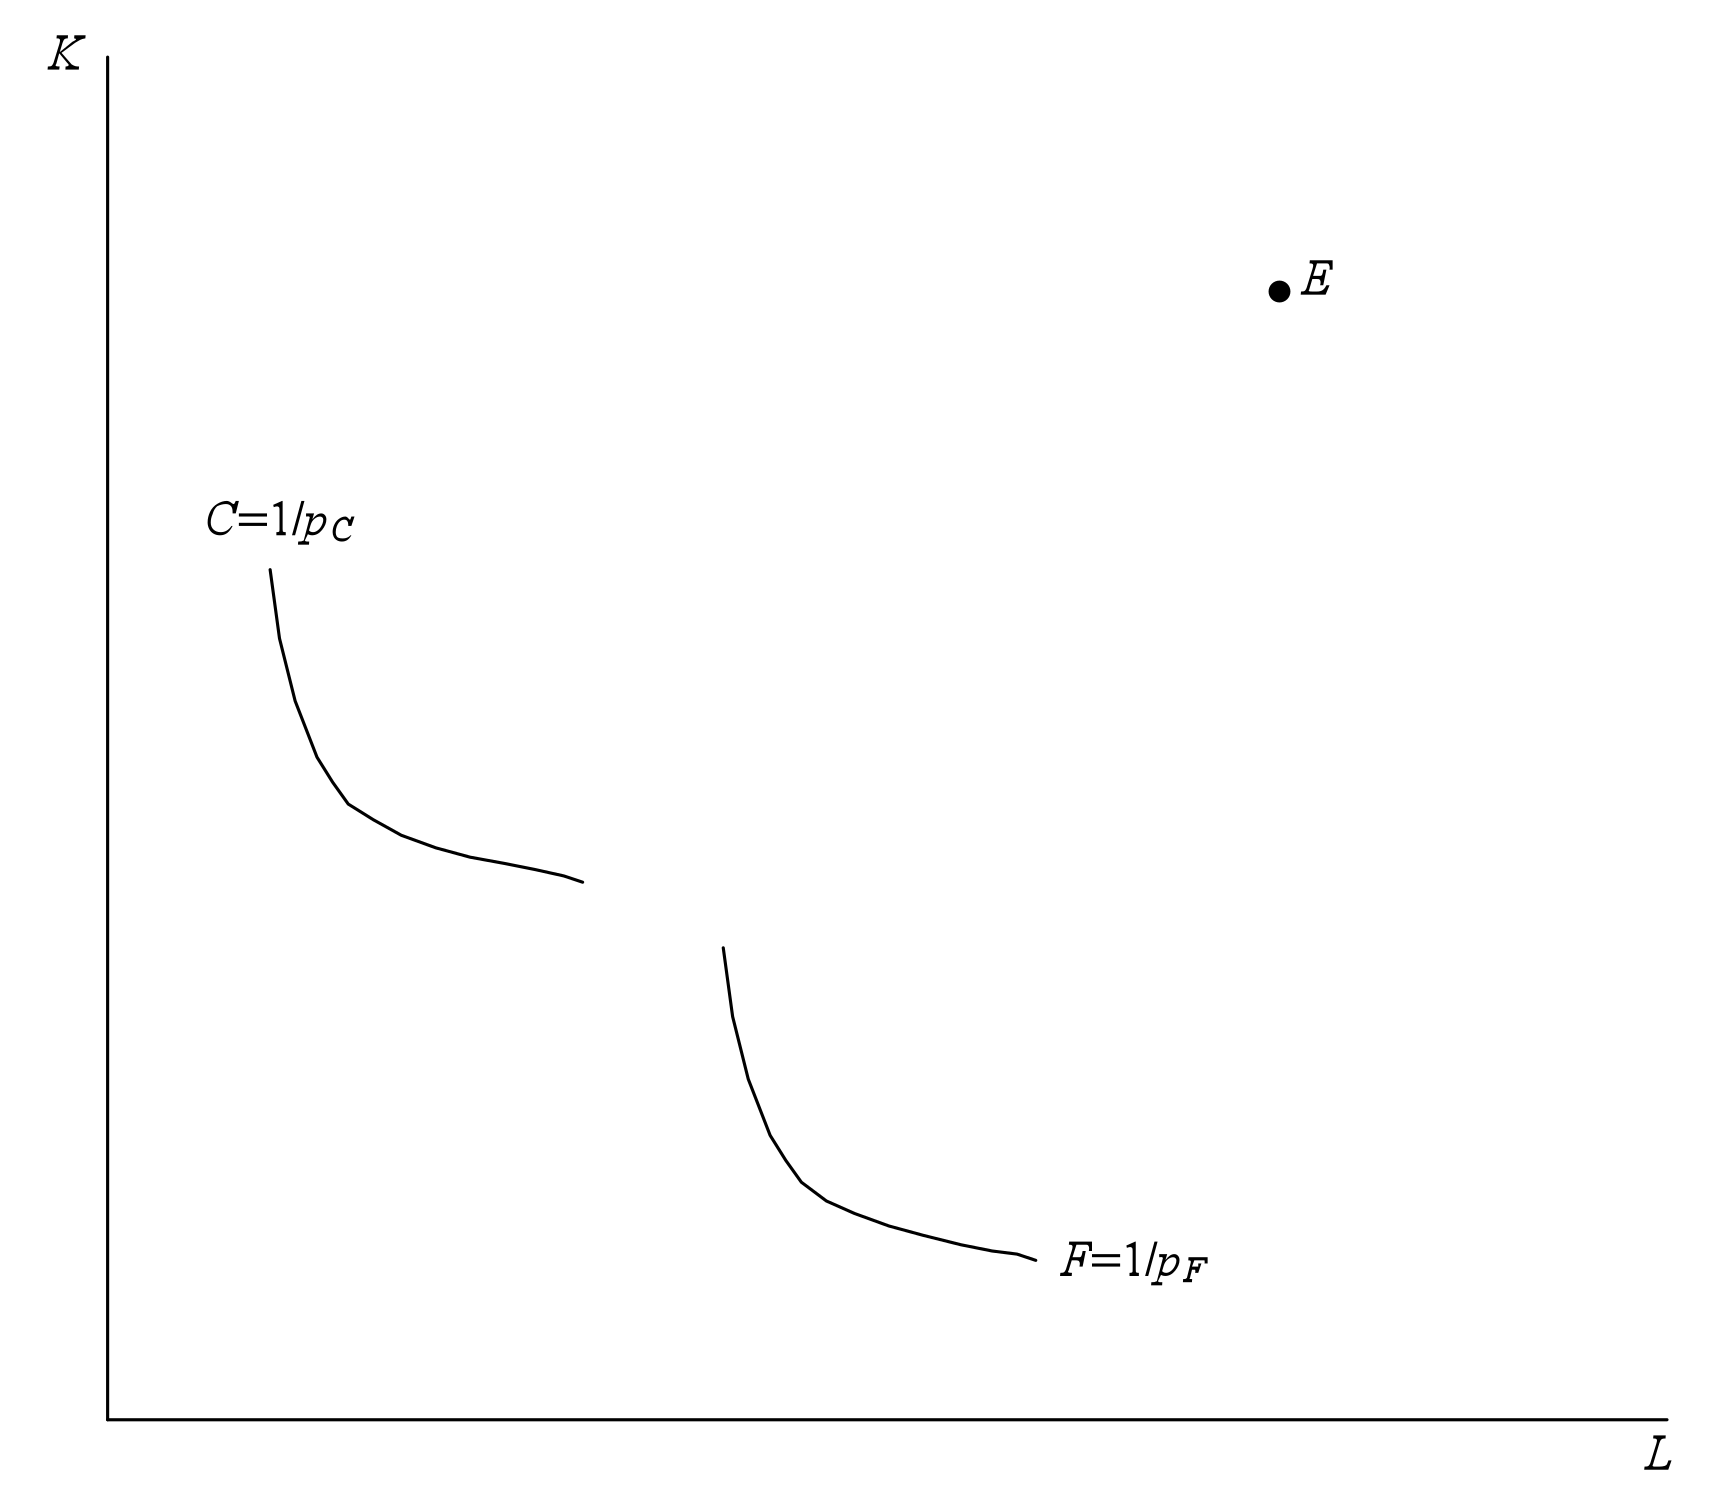
\includegraphics[scale=.5]{lerner_example.png}
  \end{figure}
\end{frame}
%--------------------------------------

%--------------------------------------
\begin{frame}{Example: how to draw a Lerner diagram}
  \begin{figure}
    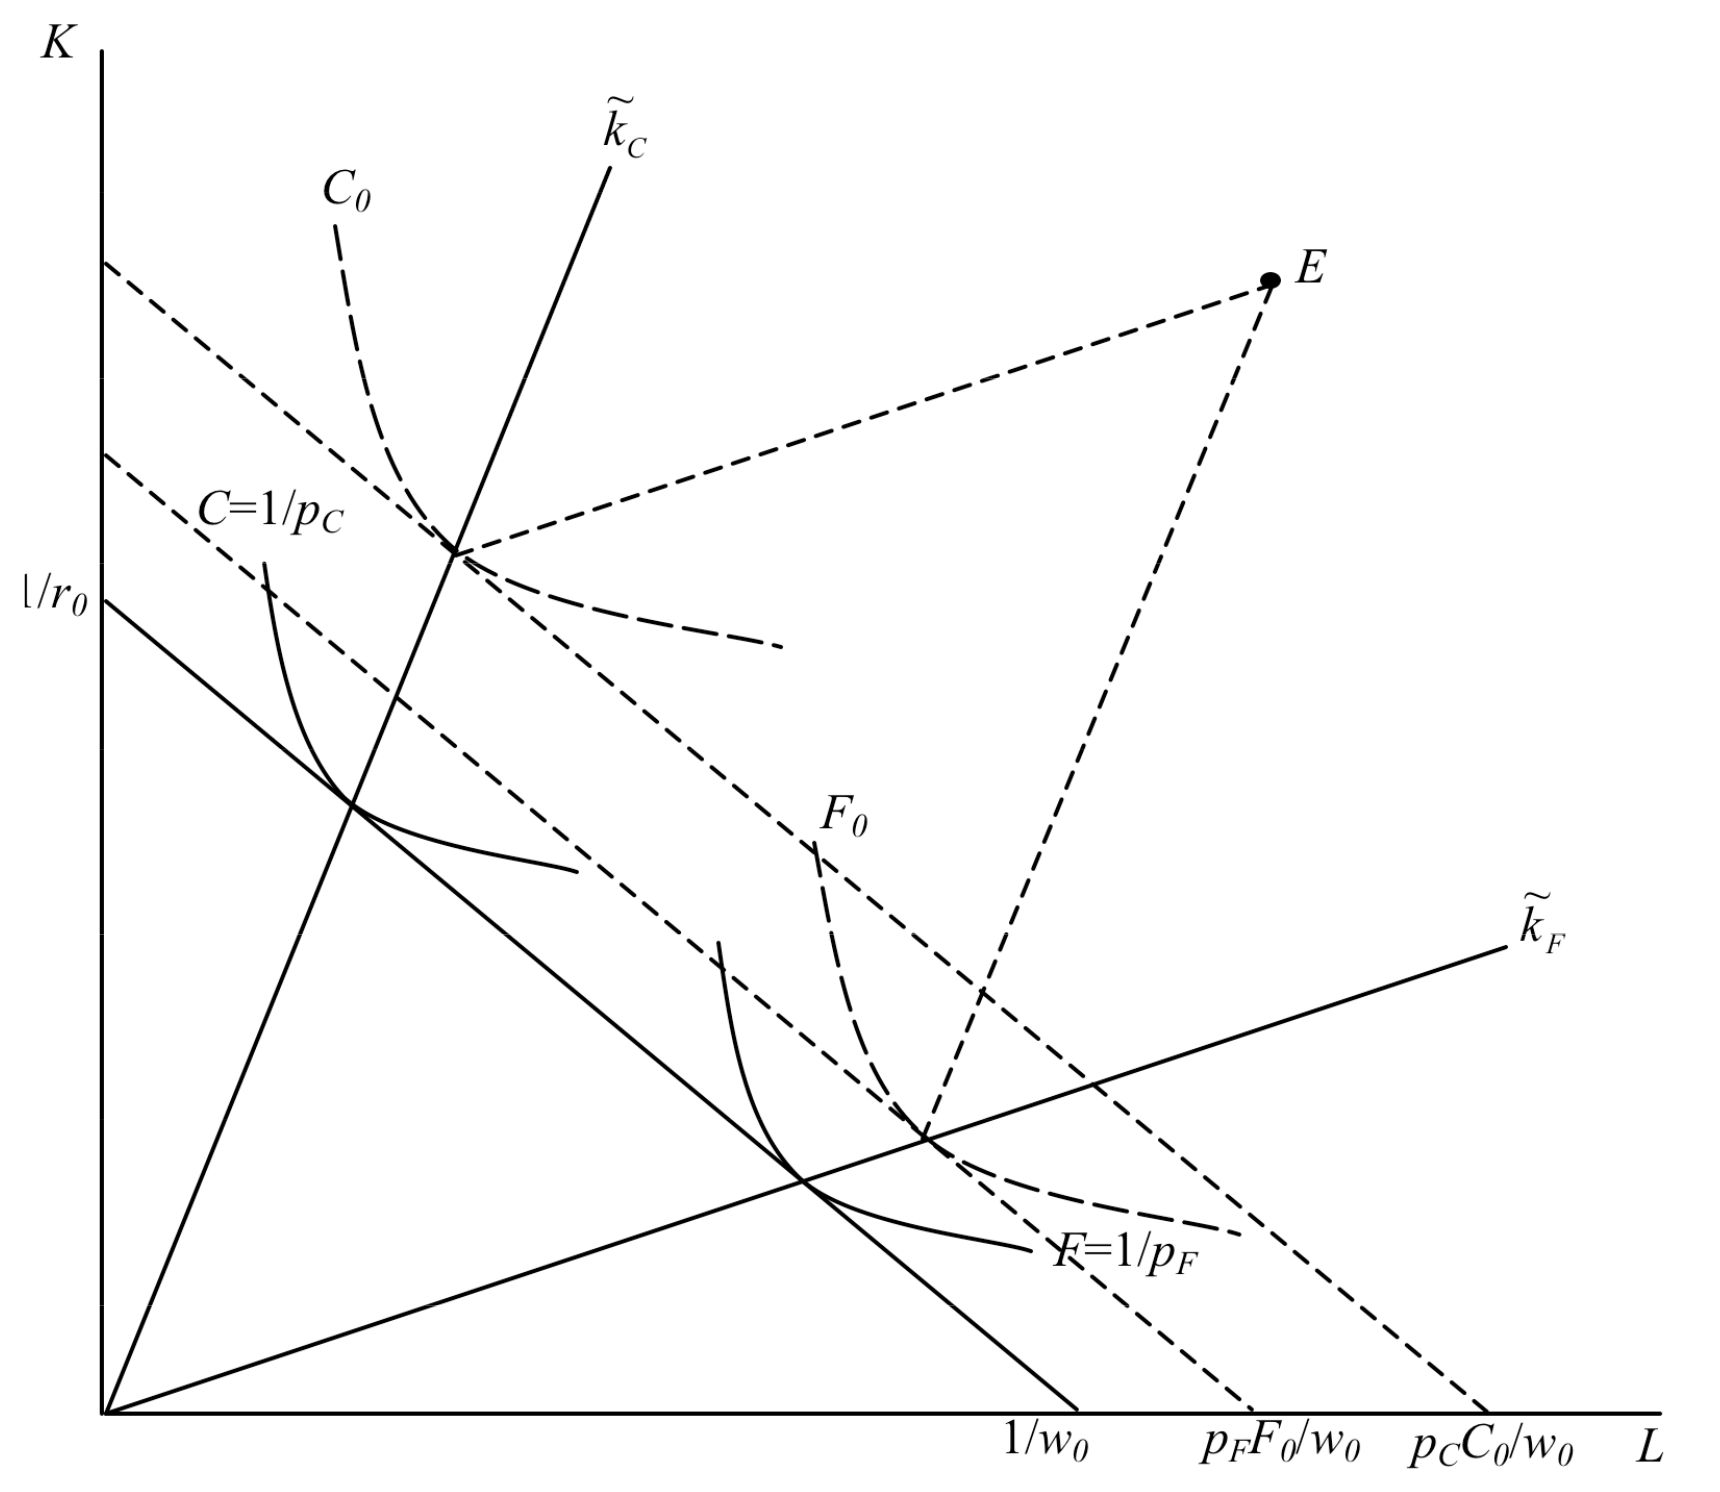
\includegraphics[scale=.5]{lerner_example2.png}
  \end{figure}
\end{frame}
%--------------------------------------

%--------------------------------------
\begin{frame}{Stolper-Samuelson theorem}
  \begin{figure}
    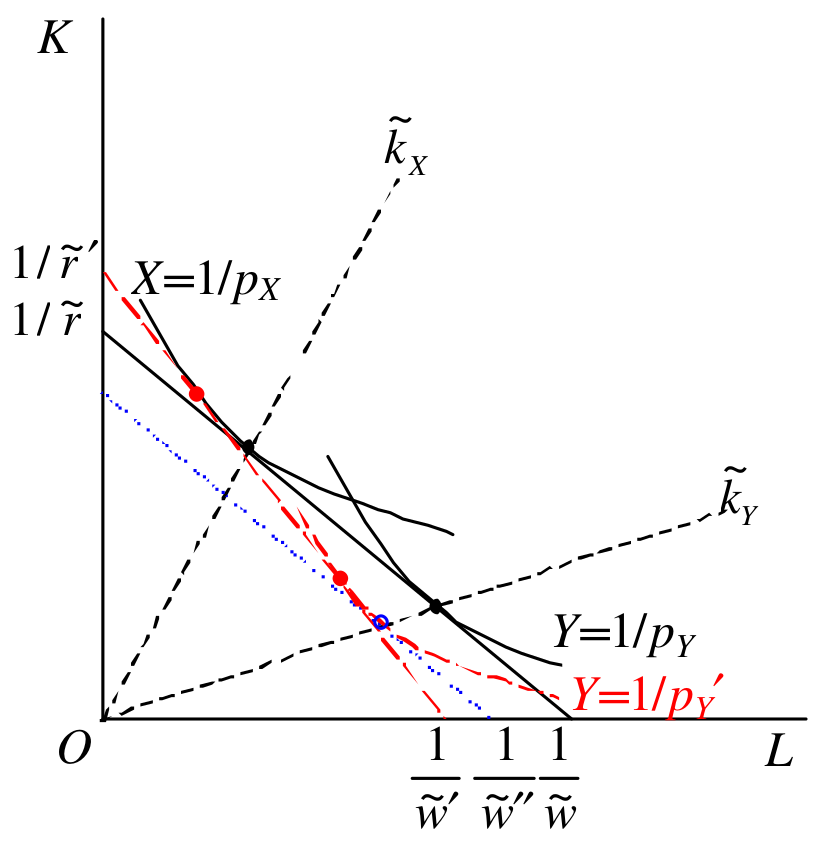
\includegraphics{lerner5.png}
  \end{figure}
\end{frame}
%--------------------------------------

%--------------------------------------
\begin{frame}
 Summarising what is happening in the figure on the previous slide
 \begin{enumerate}
   \item Increase $p_y$ holding $p_x$ constant
   \item $Y$ unit value isoquant will shift towards origin
   \item Common tangent of $X,Y$ isoquant will become steeper (red dotted line); $\frac{w}{r}$ increases
   \item Nominal wage increases, nominal rent decreases
   \item For real wage draw parallel isocost line tangent to new isoquant line which identifies wage $\widetilde{w''}$ that changed by same percentage as $p_y$
   \item Given that $\widetilde{w'}>\widetilde{w''}$ price increase causes a real wage increase
 \end{enumerate}
\end{frame}
%--------------------------------------

%--------------------------------------
\begin{frame}
 We can include more goods than factors in the HO-model and at least two types of equilibrium are possible
 \begin{enumerate}
   \item Simultaneous production of all goods
   \item Production of some goods in some countries; possibly leading to complete specialisation
 \end{enumerate}
 \medskip
 Which kind of equilibrium depends on the differences of factor endowment relative to factor intensity. 
 Here we will consider a model with three goods and two factors.
\end{frame}
%--------------------------------------

%--------------------------------------
\begin{frame}
  \begin{figure}
    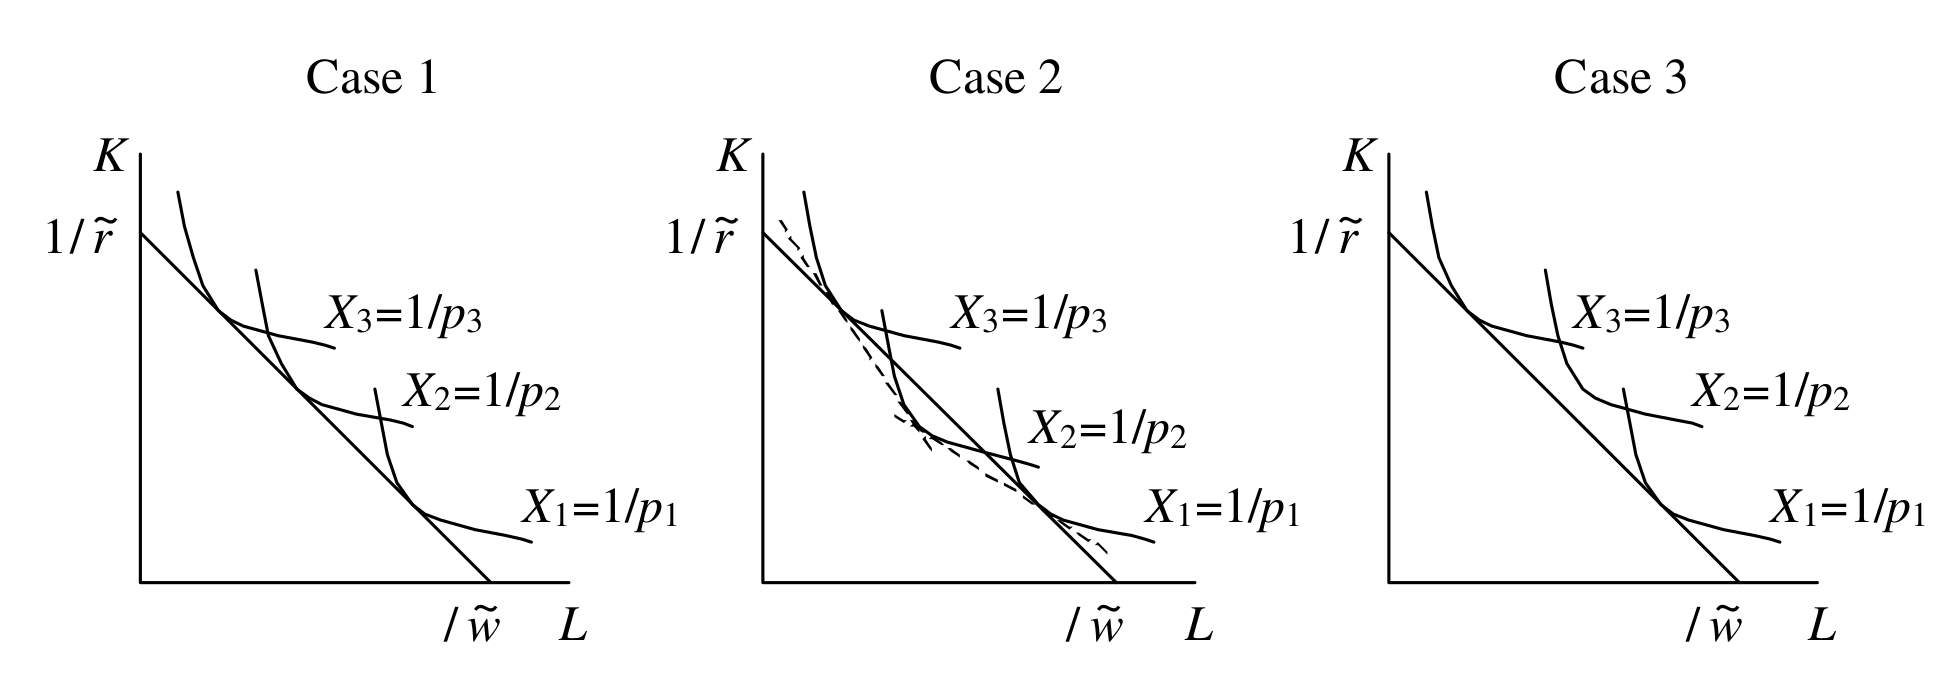
\includegraphics[scale=.7]{ho_cone.png}
  \end{figure}
\end{frame}
%--------------------------------------

%--------------------------------------
\begin{frame}
 Case 1 and 2 present two different equilibria
 \begin{enumerate}
   \item Case 1 shows the wage and rental rates consistent with breaking-even in the production of all three goods
   \item Case 2 is an equilibrium where at the given factor prices produces of $X_2$ would make a profit
   \medskip
   \item Case 3 shows a price for $X_2$ which is inconsistent with the wage and rental rate
   \begin{itemize}
      \item Production of $X_2$ is not possible anywhere in the world under free trade
    \end{itemize} 
 \end{enumerate}
\end{frame}
%--------------------------------------

%--------------------------------------
\begin{frame}{Equilibrium case 1}
  \begin{figure}
    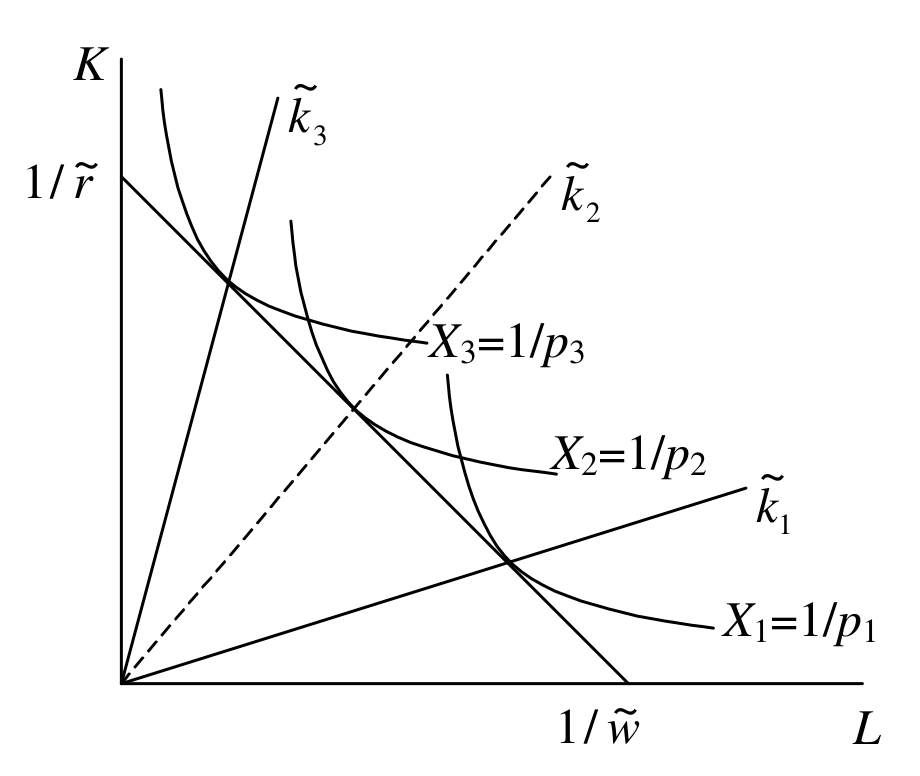
\includegraphics[scale=.7]{ho_cone2.png}
  \end{figure}  
\end{frame}
%--------------------------------------

%--------------------------------------
\begin{frame}{Equilibrium case 2}
  \begin{figure}
    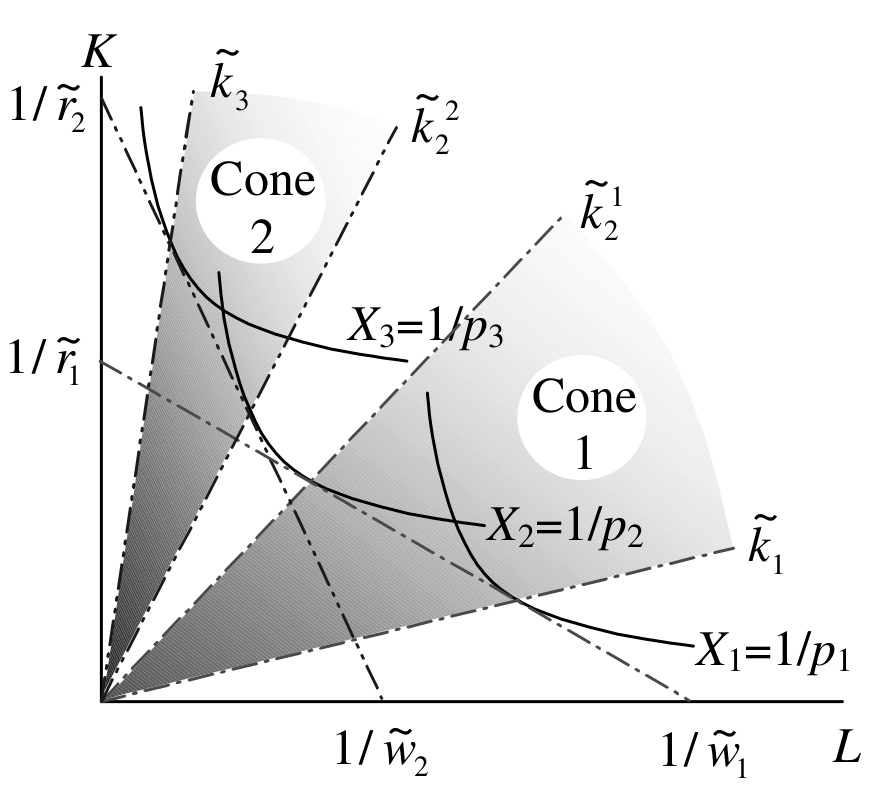
\includegraphics[scale=.7]{ho_cone3.png}
  \end{figure}
  Cone 1 has a lower capital-to-labour ratio and lower wages.
\end{frame}
%--------------------------------------

%--------------------------------------
\begin{frame}
 A remaining question is "What determines whether world equilibrium will be one or two cones?"\\
 To answer this we can use the concept of Integrated World Economy (IWE) by Dixit \& Norman (1980)
 \begin{itemize}
   \item This is a hypothetical situation in which factors are mobile across countries, which would lead to FPE   
 \end{itemize}
 \medskip
 If production factors are confined to countries but there is FPE, the IWE production of goods could be replicated 
 \begin{itemize}
   \item Resulting in a one-cone equilibrium   
 \end{itemize}
 \medskip
 Two-cone equilibrium follows when there are two sets of factor price in the world.
\end{frame}
%--------------------------------------

%--------------------------------------
\begin{frame}
  \begin{figure}
    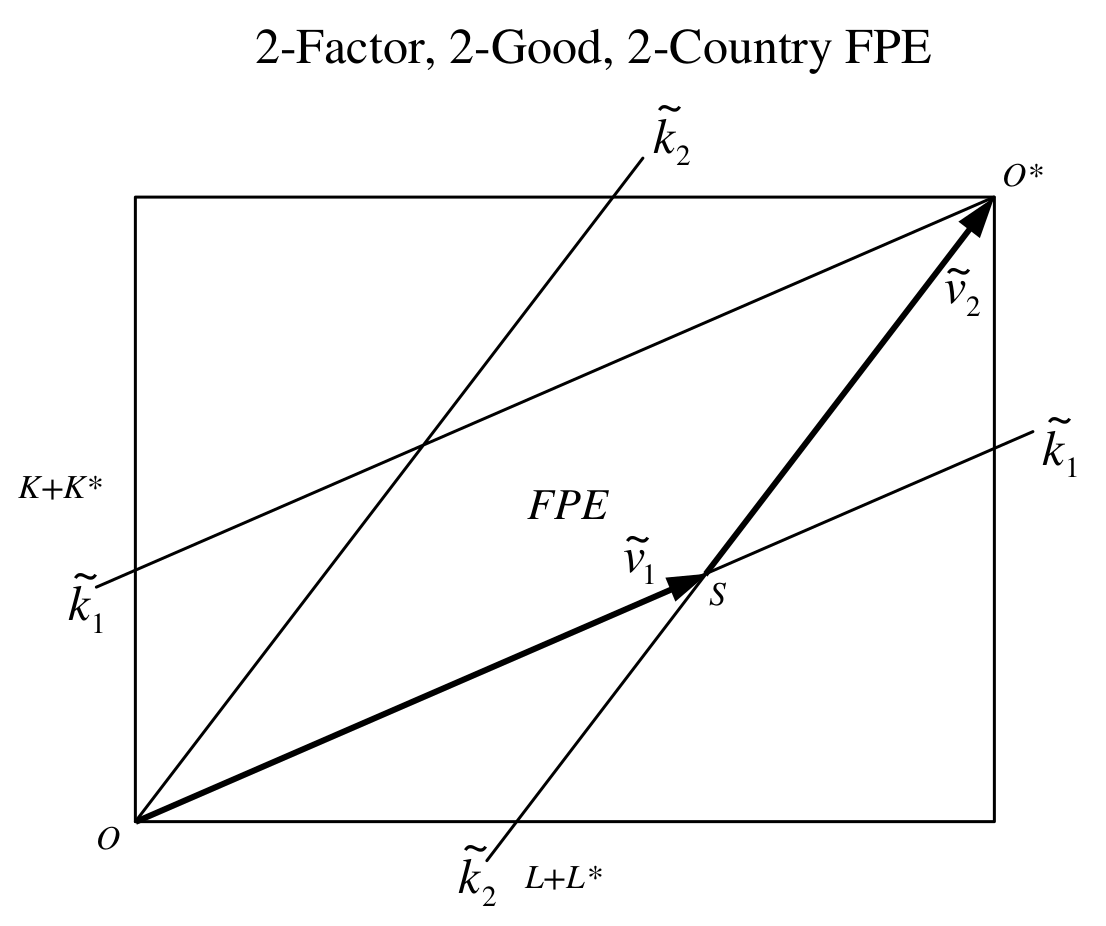
\includegraphics[scale=.7]{ho_cone4.png}
  \end{figure}
  $\widetilde{k_1}$ and $\widetilde{k_2}$ is capital employed in industry 1 and 2, $S$ is world factor allocation.\\
  Any point within the FPE parallelogram replicates the IWE with immobile factors.  
\end{frame}
%--------------------------------------

%--------------------------------------
\begin{frame}
The model can be expanded to include an additional good.\footnote{Note that $\widetilde{k_2}$ is dropped as vectors $v_i$ are strung together. \\ NB - this won't be part of the exam. }
  \begin{figure}
    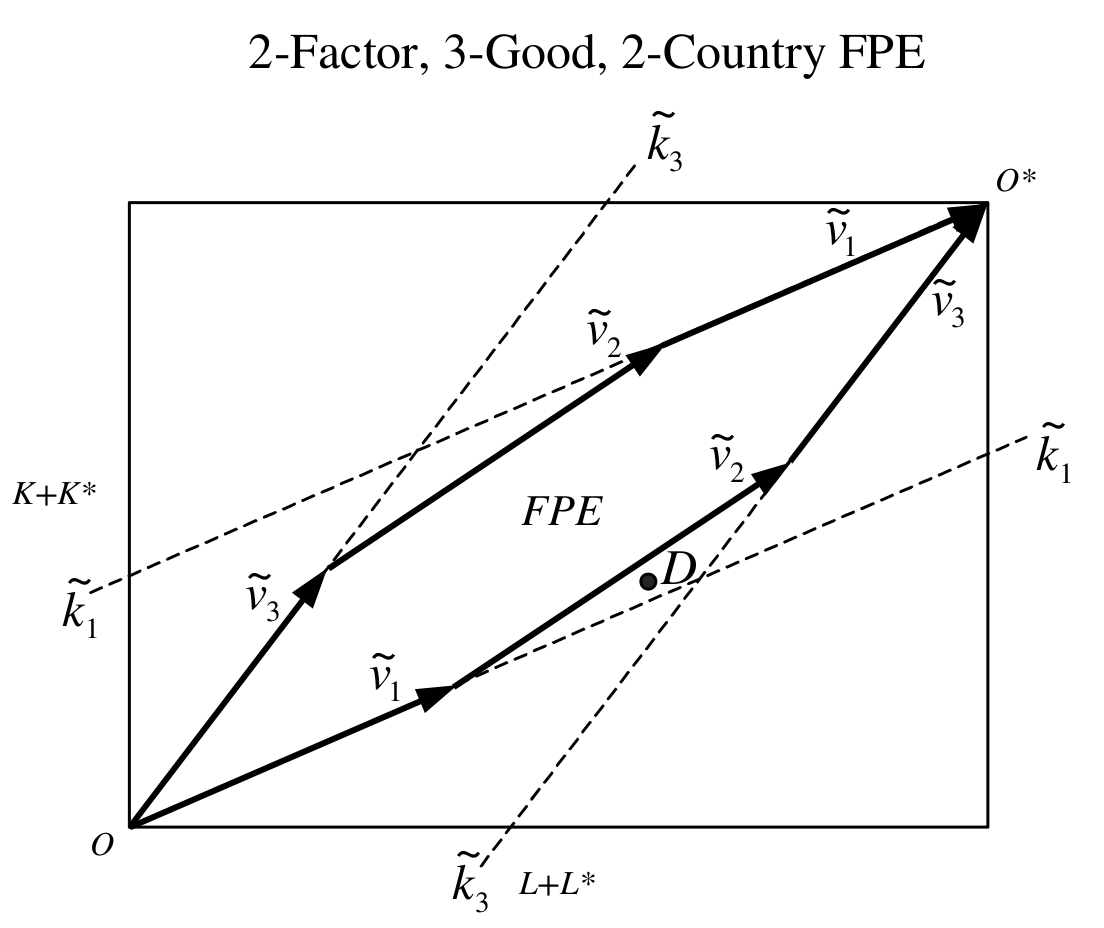
\includegraphics[scale=.7]{ho_cone5.png}
  \end{figure}
\end{frame}
%--------------------------------------

%--------------------------------------
\begin{frame}
  The HO-model does have some shortcomings, mainly related to the model's assumptions
  \begin{enumerate} 
    \item Proof of theorems requires that both countries produce both goods
    \begin{itemize}
      \item Doesn't hold when factor prices are radically different
    \end{itemize}
    \item Assumption that technology is the same everywhere
    \begin{itemize}
      \item Technological differences will affect factor productivity and thus returns to factors
    \end{itemize}
    \item Capital is completely mobile
    \item Output goods have the same price everywhere
  \end{enumerate}
  The model was formulated in 1933, and the assumptions may have been reasonable for that time but a poor reflection of the world nowadays.\\
  \bigskip
  Additionally the model ignores trade barriers and transport costs
  \begin{itemize}
    \item These may prevent output prices and factor prices equalising
  \end{itemize}
\end{frame}
%--------------------------------------

%--------------------------------------
\begin{frame}
 This leads us to the \textbf{Leontief paradox}
 \begin{quote}
  Country with higher capital to worker ratio has a lower capital to labour ratio in exports compared to imports
 \end{quote}
\end{frame}
%--------------------------------------

%--------------------------------------
\begin{frame}
  Paradox named after Leontief how computed the input-output table for the 1947 US economy
  \begin{itemize}
    \item Used input-output matrix for commodity production
    \item Combined with matrix of direct factor inputs
  \end{itemize}
  \medskip
  Calculations were based on assumption that only final goods are traded.
\end{frame}
%--------------------------------------

%--------------------------------------
\begin{frame}
 One complication with the input-output data was that Leontief had only information on capital and labour inputs in the US.
 \begin{itemize}
   \item There was no information on the direct factor inputs for the goods that the USA imported from the RoW
 \end{itemize}
 \medskip
 To deal with this he used the HO-model assumption that all countries
 \begin{itemize}
   \item Have access to the same technology
   \item Face the same factor prices
 \end{itemize}
\end{frame}
%--------------------------------------

%--------------------------------------
\begin{frame}
 He found the following capital to labour ratios (in USD per person-year)
 \begin{align*}
 Imports: & \; \frac{K}{L} = 18.200 \\
 Exports: & \; \frac{K}{L} = 13.700
 \end{align*}
 \medskip
 i.e. exports were more labour intensive than imports; this is a bit of a surprise given that the USA was the most capital abundant country at the time. 
 This also contradicts the trade pattern prediction of the HO-model.
\end{frame}
%--------------------------------------

%--------------------------------------
\begin{frame}
  Leamer (1980) pointed out that Leontief's application of HO theory was wrong if
  \begin{enumerate}
    \item Trade is unbalanced
    \item There are more than two factors in the world
  \end{enumerate}
  \medskip
  Additional explanations include 
  \begin{enumerate}
   \item Free trade lowers income of relatively scarce factor: provides lobby incentive
   \item Consumption preferences
   \item Production technologies are not identical across countries
 \end{enumerate}
\end{frame}
%--------------------------------------

%--------------------------------------
\begin{frame}
 Based on the HO-model predictions we would expect to see trade flows between developed and developing countries.  
  \begin{itemize}
    \item Western industrialised countries are relatively capital abundant, but have small labour shares
    \item Countries in the global South have plenty of labour, but not so much capital
  \end{itemize}  
\end{frame}
%--------------------------------------

%--------------------------------------
\begin{frame}
  \begin{figure}
    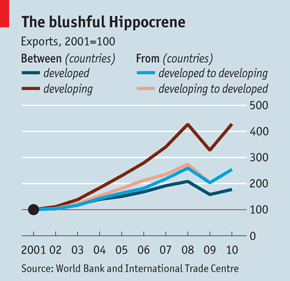
\includegraphics[scale=.7]{trade-devel-developed.png}
  \end{figure}
\end{frame}
%--------------------------------------

%--------------------------------------
\begin{frame}
Empirically there seems to be a lot of missing trade considering global factor endowments, important reasons for this are
  \begin{enumerate}
    \item Cross-country differences in technology
    \item Home bias in consumption
  \end{enumerate}
\end{frame}
%--------------------------------------

%% FIN
%------------------------------------------------------------------------------
\end{document}
